\documentclass[11pt]{article}
\usepackage[T1]{fontenc}
\usepackage[utf8]{inputenc}
\usepackage{lmodern}
\usepackage[margin=1.08in]{geometry}
\usepackage{amsmath,amssymb,amsthm,mathtools,bm}
\usepackage{microtype}
\usepackage{graphicx,booktabs,tabularx,array,float,caption}
\usepackage{setspace}
\usepackage[round,authoryear]{natbib}
\usepackage{xcolor}
\usepackage{enumitem}
\usepackage[section]{placeins}
\usepackage[hidelinks]{hyperref}
\hypersetup{pdftitle={Generative Neural Operators in Finance},
 pdfauthor={Miquel Noguer i Alonso},
 pdfsubject={DOI: 10.5281/zenodo.22714857}}
\usepackage[nameinlink,noabbrev]{cleveref}
\numberwithin{equation}{section}
\newtheorem{theorem}{Theorem}[section]
\newtheorem{proposition}[theorem]{Proposition}
\newtheorem{lemma}[theorem]{Lemma}
\newtheorem{corollary}[theorem]{Corollary}
\theoremstyle{definition}
\newtheorem{definition}[theorem]{Definition}
\newtheorem{assumption}[theorem]{Assumption}
\crefname{assumption}{assumption}{assumptions}
\Crefname{assumption}{Assumption}{Assumptions}
\newtheorem{example}[theorem]{Example}
\theoremstyle{remark}
\newtheorem{remark}[theorem]{Remark}
\newcommand{\E}{\mathbb E}
\newcommand{\R}{\mathbb R}
\newcommand{\N}{\mathbb N}
\newcommand{\Law}{\operatorname{Law}}
\newcommand{\tr}{\operatorname{tr}}
\newcommand{\Id}{\operatorname{Id}}
\newcommand{\Ran}{\operatorname{Ran}}
\newcommand{\Lip}{\operatorname{Lip}}
\newcommand{\Ptwo}{\mathcal P_2}
\newcommand{\dd}{\,\mathrm d}
\newcommand{\norm}[1]{\left\lVert#1\right\rVert}
\newcommand{\ip}[2]{\left\langle#1,#2\right\rangle}
\newcommand{\push}{_{\#}}
\newcommand{\eps}{\varepsilon}
\setlength{\emergencystretch}{2em}
\setstretch{1.08}
\captionsetup{font=small,labelfont=bf}
\setlength{\parindent}{1.25em}
\setlength{\parskip}{0pt}
\pagestyle{empty}
\setlist[itemize]{leftmargin=1.5em,itemsep=0.2em,topsep=0.35em}
\allowdisplaybreaks[1]
\newcommand{\TV}{\operatorname{TV}}
\newcommand{\CVaR}{\operatorname{CVaR}}
\newcommand{\F}{\mathcal F}
\newcommand{\Hist}{\mathsf h}
\newcommand{\softplus}{\operatorname{softplus}}
\title{\textbf{Generative Neural Operators in Finance}\\[0.35em]
\large Hidden Liquidity, Valid Market Simulation,\\ and Execution Guarantees}
\author{Miquel Noguer i Alonso\\
\small Artificial Intelligence Finance Institute (AIFI)}
\date{\today}
\begin{document}
\maketitle
\thispagestyle{empty}
\begin{center}\small\href{https://doi.org/10.5281/zenodo.22714857}{DOI: 10.5281/zenodo.22714857}\end{center}
\begin{abstract}
A generative financial model must connect latent field laws, observable market events, and decisions made from simulated paths. We establish this connection through cell-integrated event intensities, a prescribed admissible transition mechanism, and posterior transport. The main comparison transfers conditional field and posterior Wasserstein errors into total variation of the entire observable event path, with a constant independent of the numerical partition. It handles discontinuous depletion and matching events and yields bounds for fill probabilities, execution costs, tail risk, and policy regret. Hidden-regime examples distinguish latent identification from predictive equivalence, while exact posterior-randomized thinning implements the asserted observable intensity, including information from quiet intervals. For a finite observable control model, a continuation-value identity weights rate error by its economic effect. Counting-process confidence sequences turn recorded events and occupation times into simultaneous rate boxes under adaptive actions and stopping. Robust dynamic programming then certifies a policy selected from those data; a residual estimate accounts for time discretization. A separate pricing construction preserves positivity and the discounted martingale property. An adapted stopping-value bound and an equal-terminal-law counterexample show why early exercise requires control of information timing. Reproducible synthetic studies train both latent-state rate emulators and event-count-based rate networks, evaluate actual policy costs independently, and report conservative certificates alongside measured errors. A Lean project checks 40 declarations, including finite history laws, reserve conservation, policy-specific regret, robust finite-horizon comparison, and residual accumulation. Continuous-time probability, transport, filtering, and stopping arguments remain explicit written proofs. The results provide a mathematically specified route from generative approximation to decision guarantees under stated observation and intervention assumptions.
\end{abstract}
\noindent\textbf{Keywords:} generative neural operators; limit order books; hidden liquidity; nonlinear filtering; marked point processes; optimal execution; Wasserstein distance; martingale models; formal verification.
\clearpage
\setcounter{tocdepth}{2}
\tableofcontents
\clearpage
\section{Introduction}\label{sec:intro}
A market simulator is useful only through what its generated paths imply. The distribution of returns matters, but so do the probability of receiving a fill, the time needed to exhaust a queue, the price paid for a specified quantity, and the response to an action selected by a trading policy. Small errors in a displayed book representation need not imply small errors in these quantities. Depleting the final lot can change the best quote. A reserve replenishment can prevent that change. Two states with the same visible depth can therefore have different continuation laws.

Generative neural operators offer a natural representation for financial objects indexed by price, maturity, asset, or time. Their function-space formulation separates the probabilistic object from the grid on which it is computed \citep{kovachki2023,rahman2022,kerrigan2024functional}. The representation alone does not ensure that generated events are valid or that a simulated decision has approximately the right value. Those properties require a connection between field geometry, latent information, event dynamics, and decision loss.

We develop that connection in a partially observed market model. The latent state has a conditional law $\pi_t$ on a separable Hilbert space. It can describe liquidity-regime factors, unresolved order-flow intensities, and transformed reserve coordinates. It is not automatically an identifiable physical inventory. A conditional generative operator approximates $\pi_t$, and a second operator maps each latent state to a field of event-intensity densities. The densities are integrated over physical event cells and supplied to an admissible event simulator.

The central bound has the form
\begin{equation}\label{eq:intro-bound}
 \TV(\mathbb P^a_{[0,T]},\widehat{\mathbb P}^a_{[0,T]})
 \le \min\left\{1,\,
 \sqrt M\,\E^a\int_0^T
 \left[r_t+K_t\sqrt{\tau_{t,m}^2+d_{t,m}^2}\right]\dd t\right\}.
\end{equation}
Here $a$ is a common history-dependent policy, $M$ is the mass of the reference measure on event space, $r_t$ is the target-averaged conditional intensity-field error, $K_t$ is a learned latent-to-intensity sensitivity, $\tau_{t,m}$ is the unresolved posterior tail, and $d_{t,m}$ is a conditional refinement certificate. All quantities are evaluated along true histories under that policy. In particular, the theorem does not replace those histories by a passive training distribution without justification.

The error criterion in \eqref{eq:intro-bound} is strong enough to handle discontinuous path functionals. An event probability changes by at most the right-hand side. A cost taking values in $[0,B]$ changes in expectation by at most $B$ times that bound. Uniformity over a policy class gives a $2B$ multiple for model-selection regret. Tail risk introduces the explicit amplification factor $(1-\alpha)^{-1}$ for $\CVaR_\alpha$. The same guarantee does not imply a continuous value-at-risk estimate at atoms.

For decisions with a specified objective, a full-path bound can be unnecessarily conservative. We derive a continuation-value sensitivity identity and connect it to rate confidence sequences constructed from observed counts and exposures. In a finite observable state model these intervals remain valid under adaptive actions and stopping; robust dynamic programming converts the same event into a guarantee for the selected execution policy. This specialization requires observed state-action exposure and does not infer hidden reserve exposure from displayed data. Its purpose is to supply a complete statistical-to-decision chain where identification is explicit.

\subsection{Relation to existing work}
Queue-based Markov models supply a tractable mathematical description of order-book events \citep{cont2010}. Learned world-agent simulators generate market activity from data \citep{coletta2022}, while LOB-Bench evaluates distributions, conditional statistics, and event-response behavior in generated message streams \citep{nagy2025}. Our aim is to identify sufficient conditions under which such distributional approximation controls financial decisions. The paper does not claim to introduce event-driven simulation, generative market models, or hidden-state filtering.

The underlying methods are also established. Conditional transport and function-space flow matching provide generative representations \citep{hosseini2025,kerrigan2024functional}; disintegration and conditional probability supply latent posteriors \citep{kallenberg2021}; and common-Poisson coupling is a standard point-process comparison method \citep{bremaud1981}. Our contribution is the combined certificate through cell-integrated intensity fields, with an explicit separation between posterior resolution, conditional fitting, and sensitivity to latent errors. This separation makes the numerical-resolution constant and the policy-distribution requirement visible.

Financial admissibility has more than one meaning. Valid matching events concern the support of a physical market simulator. Martingale pricing concerns a separately specified pricing measure. Neural-SDE market models impose financial constraints on option dynamics \citep{cohen2021}, and VolGAN combines generative volatility modeling with scenario treatment for arbitrage constraints \citep{vuletic2024}. Risk-neutral neural operators for joint SPX--VIX term structures have also been proposed \citep{zhang2025}. We provide a simpler positive martingale construction to show exactly where an operator can enter a pricing model and to derive an adapted volatility-to-price bound. We do not identify the pricing law with the historical law or claim that a generated volatility field calibrates observed option prices.

\subsection{Main results and scope}
The principal results are: a structural validity proposition for event generation; a posterior-intensity identity and a quantitative obstruction to snapshot-only prediction; a field-to-path comparison theorem; a multiresolution posterior bound; execution and risk guarantees; a liquidity-quantile transport inequality; and an adapted martingale construction. The decision-specific extension adds event-rate confidence sequences, a robust policy sandwich, and a numerical residual allowance. A bicausal stopping comparison treats early exercise and distinguishes information timing from terminal calibration. Each result states the assumptions that make its claim meaningful.

The numerical studies include a complete reserve model with a trained rate network, exact survival-aware filtering, two exact thinning implementations, and an optimized finite class of execution deadlines. Matrix exponentiation evaluates policy errors independently of simulation. A separate queue experiment compares coupling and likelihood certificates, including an informative 99-percent tail-risk regime. A three-stream observed-event study fits rates without oracle rate labels, computes confidence boxes, and compares nominal and robust policies across three data budgets. These are controlled synthetic validations rather than exchange-data calibration or measurements of undisplayed exchange inventory. Formal verification is similarly scoped: the Lean files prove their stated mathematical declarations, and a coverage map identifies which analytic results are proved in this manuscript but not mechanized.

\section{Market state, latent fields, and valid events}\label{sec:state}
\subsection{Displayed state and the role of marks}
Fix a finite physical price grid and a finite collection of admissible order sizes. A displayed state $x$ records nonnegative integer queue sizes, relevant order identifiers if available, and any public information needed by the transition rule. A full latent state $z$ can contain reserve quantities and other predictive variables. The observed history $\Hist_{t-}$ includes the initial state, prior event times and marks, and the policy's previous actions. The filtration generated by this history is denoted $\F^O_{t-}$.

Let $\mathcal E$ be a finite mark set. A mark contains enough information that the displayed update is a deterministic map
\begin{equation}\label{eq:transition}
 x_t=\Delta(x_{t-},e_t).
\end{equation}
For example, a combined execution-and-replenishment mark must specify both executed displayed quantity and the resulting displayed replenishment. A mark that merely records an execution need not determine the next displayed state when reserves are hidden. Splitting an execution and its replenishment into two linked marks is an alternative representation, provided their timing convention is explicit.

Let $\mathcal V$ be the set of states satisfying the simulator's stated market rules. For each $x\in\mathcal V$, let $\mathcal E(x)$ contain only marks for which $\Delta(x,e)\in\mathcal V$. A simple continuous-trading model can require integer lots, nonnegative queues, cancellation quantities no larger than the relevant order, and a correctly updated best bid and ask. A limit order that crosses the opposite quote is handled by the specified matching rule. These are model requirements; a production implementation needs its own venue and feed specification. Auctions require a separate transition regime and are not represented by an unmodified continuous-trading rule.

\begin{proposition}[Structural event validity]\label{prop:validity}
Suppose $x_0\in\mathcal V$, the event process is nonexplosive on $[0,T]$, its predictable intensities are nonnegative, and the intensity of every $e\notin\mathcal E(x_{t-})$ is zero. Then $x_t\in\mathcal V$ for all $t\le T$ almost surely.
\end{proposition}
\begin{proof}
On a nonexplosive path there are finitely many jumps before $T$. Between jumps the displayed state is constant. At each jump, the sampled mark belongs to $\mathcal E(x_{t-})$ almost surely, so its transition maps a valid state to another valid state. Induction over the jump times proves the assertion.
\end{proof}

A penalty in a training loss does not imply this proposition. The support restriction belongs to the sampler and transition mechanism. Conversely, structural validity does not imply that the rates are statistically accurate.

\subsection{Reserve accounting}
At a fixed price, write $D,H\in\N$ for displayed and hidden lots. An execution consumes $q\le D$ displayed lots, and a replenishment transfers $r\le H$ hidden lots into display:
\begin{equation}\label{eq:reserve-update}
 D'=D-q+r,\qquad H'=H-r.
\end{equation}
Additional restrictions on $r$, such as replenishment only after an order's displayed peak is exhausted, are imposed by the specified admissible-mark set. They do not alter the following accounting identity.

\begin{proposition}[Execution-linked reserve conservation]\label{prop:reserve}
Under \eqref{eq:reserve-update},
\begin{equation}\label{eq:reserve-conservation}
 D'+H'=D+H-q,\qquad D',H'\ge0.
\end{equation}
For a sequence of such events with no new submissions or cancellations,
$D_n+H_n=D_0+H_0-\sum_{k<n}q_k$.
\end{proposition}
\begin{proof}
The transfer $r$ cancels when the two update equations are added. Nonnegativity follows from $q\le D$ and $r\le H$. Summing the one-step identity telescopes.
\end{proof}

Thus replenishment is a transfer, not new aggregate liquidity. Hidden submissions, cancellations, and venue-specific refresh rules can be added as separate transitions. A continuous latent field may parameterize their rates, but it does not replace integer inventory accounting. If a latent decoder rounds a real coordinate to an integer reserve, that rounding is discontinuous; one must verify the sensitivity of the resulting intensity map rather than inherit it from the pre-decoder field.

\subsection{Field-valued rates and numerical resolution}
Let $(A,\nu)$ be a finite measure space, with $M=\nu(A)<\infty$. Its coordinates may encode price offset, event type, and size. A nonnegative field
\[
 f_t(\Hist,z,\cdot)\in L^2(A,\nu)
\]
is an intensity \emph{density} with respect to $\nu$. Fix disjoint cells $(B_e)_{e\in\mathcal E}$ representing physical marks. With an observed-state feasibility mask $m_e(\Hist)\in\{0,1\}$, define
\begin{equation}\label{eq:cell-rates}
 \lambda_e(t,\Hist,z,a)
 =m_e(\Hist,a)\int_{B_e}f_t(\Hist,z,a,u)\,\nu(\dd u).
\end{equation}
The cells need not cover all of $A$; unused regions carry no sampled marks. If an admissibility condition depends on $z$, include it in the conditional intensity field and verify the required latent sensitivity for that complete field. A common observed-state mask alone does not encode every hidden-inventory constraint.

The representation in \eqref{eq:cell-rates} matters. Evaluating an $L^2$ function at an arbitrary point is not a continuous operation, and an $L^2$ equivalence class has no canonical point values. Integrating over physical cells is well defined and gives the partition-independent estimate used below. Refining numerical quadrature inside those cells leaves the physical market specification fixed. Changing the actual tick size, allowed order sizes, or matching rule changes the modeled market.

\section{Hidden liquidity as a conditional law}\label{sec:filter}
Let $\mathsf H$ be a separable real Hilbert space, and let $Z_t$ be the latent state required by the conditional rate specification. History-dependent latent dynamics can be included by enlarging the state. Assume the relevant conditional laws have finite second moments, and write
\begin{equation}
 \pi_{t-}=\Law(Z_{t-}\mid\F^O_{t-}),\qquad
 \widehat\pi_{t-}=\Law(G_\theta(\Hist_{t-},\xi)),
\end{equation}
where $\xi$ is fresh generative noise. The second expression defines a history-dependent approximate belief. Unless its update equations have been derived from a complete latent model, it should not automatically be called that model's exact Bayesian posterior.

\begin{proposition}[Observable event intensity]\label{prop:filter-rate}
Suppose $N_e$ has full-information predictable intensity
$\lambda_e(t,\Hist_{t-},Z_{t-},a_t)$, the action $a_t$ is predictable from observed history, and the rates are integrable on finite horizons. Its intensity in the observed filtration is
\begin{equation}\label{eq:observable-rate}
 \bar\lambda_e(t,\Hist_{t-},a_t)
 =\int \lambda_e(t,\Hist_{t-},z,a_t)\,\pi_{t-}(\dd z).
\end{equation}
\end{proposition}
\begin{proof}
For every bounded observed-predictable test process $\varphi_t$,
\[
 \E\int_0^T\varphi_t\dd N_e(t)
 =\E\int_0^T\varphi_t\lambda_e(t,\Hist_{t-},Z_{t-},a_t)\dd t.
\]
Conditional expectation given $\F^O_{t-}$ turns the right side into
$\E\int_0^T\varphi_t\bar\lambda_e(t,\Hist_{t-},a_t)\dd t$.
This is the compensator characterization of the observed intensity.
\end{proof}

Equation \eqref{eq:observable-rate} identifies the relevant predictive object. It generally depends on a distribution of latent states. Evaluating the rate at a posterior mean is a different operation:
$\int\lambda_e(z)\pi(\dd z)$ need not equal $\lambda_e(\int z\pi(\dd z))$.
If $\lambda_e$ is $L$-Lipschitz, the discrepancy is at most
$L\E_\pi\|Z-\E_\pi Z\|$. A posterior mean is adequate only with additional linearity, concentration, or an explicit error bound.

\subsection{A quantitative obstruction to snapshot closure}
\begin{theorem}[Snapshot prediction can have irreducible error]\label{thm:snapshot}
Consider two admissible latent specifications with the same current displayed state. Suppose their future observable counting processes over a horizon $T$ are Poisson with distinct constant rates $\lambda_0,\lambda_1$. Any single snapshot-conditioned predictive path law $Q$ satisfies
\begin{equation}\label{eq:snapshot-lower}
 \max\{\TV(P_0,Q),\TV(P_1,Q)\}
 \ge \frac12\left|e^{-\lambda_0T}-e^{-\lambda_1T}\right|.
\end{equation}
Here $P_i$ is the observable path law in latent specification $i$.
\end{theorem}
\begin{proof}
The event of no arrival has probabilities $e^{-\lambda_iT}$, hence
$\TV(P_0,P_1)\ge|e^{-\lambda_0T}-e^{-\lambda_1T}|$.
The triangle inequality implies
$\TV(P_0,P_1)\le\TV(P_0,Q)+\TV(Q,P_1)$, proving the claim.
\end{proof}

The example uses a liquidity \emph{regime}, not a reserve that remains constant despite executions. If the hidden variable is actual inventory, it must evolve according to an accounting rule such as \eqref{eq:reserve-update}. The same obstruction occurs whenever two hidden states with identical displayed observations yield different future event laws.

\begin{proposition}[Exact static-regime filter]\label{prop:poisson-filter}
Let $H\in\{0,1\}$ be a time-constant latent regime with prior
$\mathbb P(H=1)=p\in(0,1)$. Conditional on $H=i$, observed marked counts have constant positive intensities $\lambda_i(e)$. Write
$\Lambda_i=\sum_e\lambda_i(e)$. Then
\begin{equation}\label{eq:logodds}
 \log\frac{p_t}{1-p_t}
 =\log\frac p{1-p}
 +\sum_{k:t_k\le t}\log\frac{\lambda_1(e_k)}{\lambda_0(e_k)}
 -t(\Lambda_1-\Lambda_0).
\end{equation}
\end{proposition}
\begin{proof}
The marked point-process likelihood under regime $i$ is proportional to
$e^{-t\Lambda_i}\prod_{k:t_k\le t}\lambda_i(e_k)$.
The likelihood ratio times the prior odds gives the posterior odds. Taking logarithms proves \eqref{eq:logodds}.
\end{proof}

The survival term is essential: observing no arrival is information about intensity. A method that updates only at trades but ignores elapsed time does not implement this filter.

\subsection{Identifiability, prediction, and interventions}
Latent identification is stronger than predictive sufficiency. If two latent descriptions induce the same observable path law, observable data cannot distinguish them, however accurate the simulator becomes. An operational definition of hidden liquidity should therefore specify whether its target is physical undisplayed quantity, a posterior for that quantity under a structural model, or a latent variable that predicts replenishment and price response.

There is a second identification issue for trading policies. Suppose a passive dataset contains only action $a=0$. Two models can agree on
$\lambda(t,\Hist,z,0)$ for every observed history and assign different rates to $a=1$. They have identical passive likelihoods and different counterfactual execution laws. No bound for a newly optimized policy follows from passive fit alone. The uniform-policy result below assumes accurate action-dependent rates on the histories and actions generated by the policy class. Randomized interventions, a valid structural model, or other justified identification conditions must provide that information.

\section{From field error to observable path error}\label{sec:main}
We use the convention
\[
 \TV(P,Q)=\sup_{B}|P(B)-Q(B)|\in[0,1].
\]
For finite sample spaces it equals $\frac12\sum_\omega|P(\omega)-Q(\omega)|$.
The factor $\frac12$ is essential for the execution constants below.

\begin{assumption}[A common admissible simulator]\label{ass:simulator}
The true and learned models have the same initial observed state, the same finite mark set, and the same deterministic transition rule $\Delta$. A common predictable policy $a_t=a(t,\Hist_{t-})$ supplies actions. On the finite horizon $[0,T]$, both observable intensity functionals are measurable and bounded by a finite deterministic envelope. Their point-process constructions are unique in law. The learned functional is defined on every true history needed in the comparison, including histories absent from training.
\end{assumption}

A bounded envelope is a convenient sufficient condition for nonexplosion and common thinning. The comparison extends to nonexplosive locally bounded models by stopping and integrable limits, but the bounded version is all that is required here. A randomized policy is covered by adding a shared random seed to the initial observed information.

\begin{lemma}[Cell integration controls event-rate error]\label{lem:cells}
For $f,g\in L^2(A,\nu)$, disjoint measurable cells $(B_e)$, and common masks $m_e\in[0,1]$,
\begin{equation}\label{eq:cell-contraction}
 \sum_e\left|m_e\int_{B_e}(f-g)\dd\nu\right|
 \le\|f-g\|_{L^1(\nu)}
 \le\sqrt M\,\|f-g\|_{L^2(\nu)}.
\end{equation}
The constant does not depend on the number of cells.
\end{lemma}
\begin{proof}
The absolute integral on each cell is bounded by the integral of the absolute value. Summing over disjoint cells and using $m_e\le1$ gives the first inequality. Cauchy--Schwarz applied to $|f-g|$ and the constant function $1$ gives the second.
\end{proof}

\begin{lemma}[Latent uncertainty and conditional fitting]\label{lem:posterior}
Fix time, observed history, and action. Let true and learned rates be obtained from fields $f(z),\widehat f(z)$ by the same cell integration and mask. Suppose
\begin{equation}\label{eq:field-lip}
 \|\widehat f(z)-\widehat f(z')\|_{L^2(\nu)}
 \le K\|z-z'\|_{\mathsf H}.
\end{equation}
Let $\pi,\widehat\pi\in\Ptwo(\mathsf H)$ and define
\[
 r=\int\|f(z)-\widehat f(z)\|_{L^2(\nu)}\,\pi(\dd z),
 \qquad \kappa=W_2(\pi,\widehat\pi).
\]
Then the posterior-averaged observable intensities satisfy
\begin{equation}\label{eq:rate-error}
 \sum_e|\bar\lambda_e-\widehat{\bar\lambda}_e|
 \le\sqrt M\,(r+K\kappa).
\end{equation}
\end{lemma}
\begin{proof}
Insert the intermediate rate obtained by averaging $\widehat f$ under $\pi$.
For the first difference, integrate \eqref{eq:cell-contraction} under $\pi$, obtaining $\sqrt M r$.
For the second, let $(Z,\widehat Z)$ have any coupling of $\pi,\widehat\pi$. Jensen's inequality for absolute value, \Cref{lem:cells}, and \eqref{eq:field-lip} give
\[
 \sum_e\left|\E\widehat\lambda_e(Z)-\E\widehat\lambda_e(\widehat Z)\right|
 \le\sqrt M K\,\E\|Z-\widehat Z\|
 \le\sqrt M K\,(\E\|Z-\widehat Z\|^2)^{1/2}.
\]
Take the infimum over couplings. The result only needs $W_1$; using $W_2$ permits the orthogonal posterior certificate of the next section.
\end{proof}

\begin{theorem}[Path comparison through observable intensities]\label{thm:path}
Under \Cref{ass:simulator}, let
\begin{equation}
 \delta_t(\Hist)=\sum_e
 |\bar\lambda_e(t,\Hist,a_t)-\widehat{\bar\lambda}_e(t,\Hist,a_t)|.
\end{equation}
The observable path laws, including the event times, marks, and displayed states, satisfy
\begin{equation}\label{eq:path-tv}
 \TV(\mathbb P^a_{[0,T]},\widehat{\mathbb P}^a_{[0,T]})
 \le \min\left\{1,\E^a\int_0^T\delta_t(\Hist_{t-})\dd t\right\}.
\end{equation}
If $\delta_t(\Hist)\le b(t)$ for a deterministic nonnegative integrable function on every common history, then also
\begin{equation}\label{eq:uniform-path-tv}
 \TV(\mathbb P^a_{[0,T]},\widehat{\mathbb P}^a_{[0,T]})
 \le 1-\exp\left(-\int_0^T b(t)\dd t\right).
\end{equation}
\end{theorem}
\begin{proof}
For each mark use a common Poisson random measure on time and a nonnegative auxiliary coordinate, accepting a point when its auxiliary coordinate is below the respective intensity. Continue both constructions after they disagree, using their own histories. Each marginal has its prescribed law.

Let $\sigma$ be the first time the accepted marked histories differ. Before $\sigma$ the observed states, actions, and histories coincide. For mark $e$, disagreement occurs when the auxiliary coordinate lies between the two intensities, an interval of length
$|\bar\lambda_e-\widehat{\bar\lambda}_e|$. Consequently, the first-disagreement counting process has compensator
\[
 \int_0^{T\wedge\sigma}\delta_t(\Hist_{t-})\dd t.
\]
It follows that
\[
 \mathbb P(\sigma\le T)
 =\E\int_0^T\mathbf1_{\{t<\sigma\}}\delta_t(\Hist_{t-})\dd t
 \le\E^a\int_0^T\delta_t(\Hist_{t-})\dd t.
\]
After dropping the indicator, the expectation is under the true marginal. The probability that two coupled paths differ bounds their total variation, proving \eqref{eq:path-tv}.

For the deterministic envelope, put $S(t)=\mathbb P(\sigma>t)$. The compensator identity gives an absolutely continuous survival function with
$-S'(t)=\E[\mathbf1_{\{t<\sigma\}}\delta_t]\le b(t)S(t)$ almost everywhere.
The integrating-factor inequality yields
$S(T)\ge\exp(-\int_0^T b)$, proving \eqref{eq:uniform-path-tv}.
\end{proof}

No metric regularity of $\Delta$ enters the proof. A discontinuous price change after depletion is harmless on the event that the marked histories coincide. Conversely, the result does not compare two different matching engines: if the same mark causes different updates, agreement of intensities alone is insufficient.

\begin{theorem}[The generative-operator market certificate]\label{thm:main}
Under \Cref{ass:simulator}, assume the field representation and hypotheses of \Cref{lem:posterior} hold predictably along true histories, with finite
$\E^a\int_0^T\sqrt M(r_t+K_t\kappa_t)\dd t$. Then
\begin{equation}\label{eq:main}
 \TV(\mathbb P^a_{[0,T]},\widehat{\mathbb P}^a_{[0,T]})
 \le\min\left\{1,\sqrt M\,\E^a\int_0^T(r_t+K_t\kappa_t)\dd t\right\}.
\end{equation}
If implemented observable rates have an additional $\ell^1$ error
$q_t(\Hist)$ relative to the rates just described, add
$\E^a\int_0^T q_t(\Hist_{t-})\dd t$ inside the minimum.
\end{theorem}
\begin{proof}
Insert \eqref{eq:rate-error} into \eqref{eq:path-tv}. For the implemented rates use the triangle inequality for their $\ell^1$ difference before applying the same comparison.
\end{proof}

The extra term can include numerical quadrature, posterior Monte Carlo, and other rate-evaluation errors only when an appropriate bound for the actual predictable implementation is available. A discrete-time sampler that rounds all event times to a grid can have a path law singular to a continuous-time event law. Such time rounding is not automatically represented by a small rate perturbation.

\subsection{Exact posterior randomization at thinning proposals}\label{sec:posterior-thinning}
There is a direct implementation of the averaged intensity that does not hold a sampled latent rate during a waiting interval. It uses fresh randomness at every proposal, including proposals that are rejected.

\begin{proposition}[Posterior-randomized thinning]\label{prop:posterior-thinning}
For each mark $e$, let $c_e>0$ be a deterministic bound for
$\widehat\lambda_e(t,h,z,a)$ on every required time, history, action, and latent state. Generate independent Poisson proposals of rate $c_e$. At a proposal time $t$, evaluate the history-dependent kernel $\widehat\pi_{t-}(h)$, draw a fresh $Z\sim\widehat\pi_{t-}(h)$ and independent $V\sim\mathrm{Unif}(0,1)$, and accept $e$ when
\begin{equation}\label{eq:posterior-thinning}
 V\le\widehat\lambda_e(t,h,Z,a)/c_e.
\end{equation}
The accepted process has observable intensity
$\int\widehat\lambda_e(t,h,z,a)\widehat\pi_{t-}(h,\dd z)$.
The same conclusion holds with one proposal stream of rate $c$ whenever
$\sum_e\widehat\lambda_e\le c$, by selecting mark $e$ with probability
$\widehat\lambda_e/c$ and rejecting the remaining probability.
\end{proposition}
\begin{proof}
Regard each proposal as carrying independent uniform marks that randomize the latent kernel and acceptance decision. Conditional on the observable past, its acceptance probability for $e$ is
$\int\widehat\lambda_e(t,h,z,a)\widehat\pi_{t-}(h,\dd z)/c_e$.
The marked-Poisson compensator formula multiplies this probability by the proposal rate $c_e$. Boundedness gives nonexplosion, and \Cref{ass:simulator} identifies the resulting law. The one-stream construction replaces the Bernoulli mark by a categorical mark with the displayed probabilities and the same compensator calculation.
\end{proof}

The kernel is evaluated at the current time even when no market event has occurred. In a finite hidden model with no unobserved transitions between observed jumps, the posterior weights evolve over a quiet interval of length $u$ as
\begin{equation}\label{eq:survival-filter}
 p_s(u)=\frac{p_s(0)e^{-\Lambda_su}}{\sum_vp_v(0)e^{-\Lambda_vu}},
 \qquad\Lambda_s=\sum_e\lambda_e(s).
\end{equation}
After an observed mark, multiply by its conditional rate, apply its hidden-state transition, and normalize. Rejected proposals are internal simulation events and are not added to the observed history. For hidden transitions between events, the exponential in \eqref{eq:survival-filter} is replaced by the appropriate killed transition semigroup.

One exact posterior draw per proposal suffices: it introduces no Monte Carlo rate bias. An approximate posterior or an approximate acceptance rate still incurs the corresponding errors in \Cref{thm:main}. Holding a single draw through an exponential waiting time instead gives a different construction unless a coherent latent model and its filter are maintained. For rates $1$ and $4$ with equal prior weights, the correct latent-mixture survival at time one is
$\tfrac12(e^{-1}+e^{-4})=0.193097540$.
The changing posterior in \eqref{eq:survival-filter} reproduces it; freezing the averaged rate at $2.5$ gives $e^{-2.5}=0.082084999$.

\subsection{The likelihood route and when it is preferable}\label{sec:kl}
Under absolute continuity, the standard point-process likelihood offers a second comparison \citep{bremaud1981}. Assume the same initial law, common event representation, bounded predictable rates, and that the likelihood ratio is valid and integrable. In particular, a strictly positive learned rate on every feasible mark with positive true rate is a convenient sufficient support condition. Then
\begin{equation}\label{eq:path-kl}
 D_{\rm KL}(\mathbb P^a\|\widehat{\mathbb P}^a)
 =\E^a\int_0^T\sum_e\left[
 \bar\lambda_e\log\frac{\bar\lambda_e}{\widehat{\bar\lambda}_e}
 -\bar\lambda_e+\widehat{\bar\lambda}_e\right]\dd t.
\end{equation}
The convention is $0\log(0/q)=0$; a positive true rate against a zero learned rate yields an infinite contribution. Taking the logarithm of the likelihood ratio and replacing each expected counting integral by its compensator proves \eqref{eq:path-kl}. Pinsker's inequality gives the additional bound
\begin{equation}\label{eq:pinsker}
 \TV(\mathbb P^a,\widehat{\mathbb P}^a)
 \le\min\{1,\sqrt{D_{\rm KL}(\mathbb P^a\|\widehat{\mathbb P}^a)/2}\}.
\end{equation}
These are classical likelihood inequalities, not additional novelty claims.

If $\widehat\lambda=(1+\theta)\lambda$ on a set of marks, its KL integrand equals
$\lambda[\theta-\log(1+\theta)]
=\lambda\theta^2/2+O(\lambda|\theta|^3)$.
Thus the KL bound scales as $|\theta|\sqrt{\E\int\lambda}/2$ to first order, whereas the common-event $L^1$ bound scales as $|\theta|\E\int\lambda$. Neither dominates universally. The $L^1$ route handles support mismatch and separates field, posterior, and implementation errors without a denominator containing a small rate. When both apply, use the smaller certificate. A terminal-state TV measurement is not a full-path TV measurement and should not be used to declare either path bound sharp.

\subsection{A mean posterior bound from a coupled latent model}\label{sec:posterior-stability}
The following finite-state observation is useful when the learned filter is derived from a complete simulator, as in \Cref{sec:complete-model}.

\begin{proposition}[Posterior stability in expectation]\label{prop:filter-stability}
Let $P,Q$ be joint laws of observed history $Y$ and a finite hidden state $S$. Let $p(\cdot\mid Y),q(\cdot\mid Y)$ be posterior versions, with $q$ defined on all required $P_Y$ histories. Then
\begin{equation}\label{eq:mean-posterior-tv}
 \E_{P_Y}\TV(p(\cdot\mid Y),q(\cdot\mid Y))\le2\TV(P,Q).
\end{equation}
For a common finite hidden-state model with equal initial law, the same marked transition maps, and total outgoing rate discrepancy bounded by $\epsilon_\lambda$, common-event coupling gives
$\TV(P_t,Q_t)\le1-e^{-\epsilon_\lambda t}$ for the joint history and current hidden state. If the hidden-state metric has diameter $D$, then
\begin{equation}\label{eq:mean-posterior-wone}
 \E_P W_1(\pi_{t-},\widehat\pi_{t-})
 \le2D(1-e^{-\epsilon_\lambda t}).
\end{equation}
\end{proposition}
\begin{proof}
Use a common dominating measure for the observed-history marginals, with densities $a,b$. The triangle inequality gives
$\sum_s|a p_s-a q_s|\le\sum_s|a p_s-b q_s|+|a-b|$.
Integrate and divide by two. The resulting terms are $\TV(P,Q)$ and $\TV(P_Y,Q_Y)$, and marginalization contracts TV. For the dynamic statement couple equal full initial states and use common-event thinning; prior to disagreement the full histories and transitions agree. Finally a maximal coupling on the finite state set gives $W_1\le D\TV$, proving \eqref{eq:mean-posterior-wone}.
\end{proof}

This is an average over true histories, exactly the type of quantity used by \Cref{thm:main}. It is not a uniform pathwise filter bound: rare observed histories can have much larger posterior discrepancies. The $W_1$ form of \Cref{lem:posterior} is preferable here to replacing $W_1$ by $W_2$ and introducing a square-root loss for small finite-state errors.


\subsection{Finite posterior sampling}
Suppose the learned averaged rate is estimated at a fixed history from $N$ independent draws $\widehat Z_i\sim\widehat\pi$. For finite marks,
\begin{equation}\label{eq:mc-rates}
 \E\sum_e\left|
 \frac1N\sum_{i=1}^N\widehat\lambda_e(\widehat Z_i)
 -\E_{\widehat\pi}\widehat\lambda_e(\widehat Z)\right|
 \le \frac1{\sqrt N}\sum_e
 \sqrt{\operatorname{Var}_{\widehat\pi}(\widehat\lambda_e(\widehat Z))}.
\end{equation}
Indeed, each sample mean has variance divided by $N$, and Cauchy--Schwarz bounds its mean absolute error. This is a conditional expectation bound, not a deterministic uniform-in-history bound. Reusing particles or drawing them only at decision times changes their temporal dependence. To apply \Cref{thm:main}, include their randomness in the predictable simulation construction and verify the integrated error under that construction.

\subsection{What resolution independence does and does not imply}
The constant $\sqrt M$ is stable when physical cells are subdivided or quadrature is refined using a fixed reference measure. If instead an unweighted vector norm assigns unit mass to every newly added coordinate, $M$ grows with the representation. The resulting $\sqrt{|\mathcal E|}$ factor is then a change of geometry, not a contradiction.

Neither \Cref{lem:cells} nor \Cref{thm:main} proves that a coarse book path is an autonomous projection of a fine book path. Fine events can change coarse transition probabilities, and hidden reserves can change future displayed behavior. The theorem controls the law generated at the stated physical event resolution. A claim of pathwise consistency across different market resolutions requires an additional compatible transition construction.

\section{A posterior certificate from conditional refinement}\label{sec:refine}
The previous theorem separates posterior error from intensity fitting. We now derive a posterior error bound directly from conditional detail laws, orthogonality, and Wasserstein coupling. The proof below is self-contained; its application along financial histories additionally requires a predictable family of posteriors and error bounds.

Fix a time and observed history. Let $P_j$ be nested finite-rank orthogonal projections on $\mathsf H$, with $P_{-1}=0$ and $P_j\to I$ strongly. Set
$E_j=\operatorname{Ran}(P_j-P_{j-1})$ and let $\mu_j=(P_j)_\#\pi$.
Disintegrate the target posterior into conditional detail laws
\[
 K_j(x,\cdot)=\Law((P_j-P_{j-1})Z\mid P_{j-1}Z=x).
\]
The learned generator appends a detail drawn from $\widehat K_j(\widehat x,\cdot)$ to its previously generated context. Its level-$j$ law is $\widehat\mu_j$ and is supported on $\operatorname{Ran}P_j$. Use Borel versions of the detail kernels with finite second moments on the contexts involved in the comparison.

\begin{assumption}[Conditional errors and learned sensitivity]\label{ass:refine}
For every retained level, let
\begin{align}
 \eps_j^2&=\int W_2^2(K_j(x),\widehat K_j(x))\,\mu_{j-1}(\dd x)<\infty,
 \label{eq:eps}\\
 W_2(\widehat K_j(x),\widehat K_j(y))&\le L_j\|x-y\|,
 \label{eq:detail-lip}
\end{align}
where $L_j\ge0$ applies to every context needed in the comparison. Set $L_0=0$ and $\mu_{-1}=\delta_0$. These quantities concern conditional population laws, not raw empirical training loss.
\end{assumption}

\begin{theorem}[Orthogonal posterior certificate]\label{thm:posterior-certificate}
Under \Cref{ass:refine}, define
\begin{equation}\label{eq:recurrence}
 d_{-1}=0,\qquad d_j^2=d_{j-1}^2+(\eps_j+L_jd_{j-1})^2.
\end{equation}
Then
\begin{equation}\label{eq:posterior-certificate}
 W_2^2(\pi,\widehat\mu_m)
 =\tau_m^2+W_2^2(\mu_m,\widehat\mu_m)
 \le\tau_m^2+d_m^2,\qquad
 \tau_m^2=\E_\pi\|(I-P_m)Z\|^2.
\end{equation}
Furthermore,
\begin{equation}\label{eq:exp-certificate}
 d_m^2\le
 2\sum_{j=0}^m\eps_j^2\prod_{k=j+1}^m(1+2L_k^2)
 \le2\exp\left(2\sum_{k=1}^mL_k^2\right)\sum_{j=0}^m\eps_j^2.
\end{equation}
\end{theorem}
\begin{proof}
Couple the previous target and generated contexts $(X,\widehat X)$ with
$D=(\E\|X-\widehat X\|^2)^{1/2}$. Conditional on $(X,\widehat X)=(x,y)$, choose optimal couplings between $K_j(x)$ and $\widehat K_j(x)$, and between $\widehat K_j(x)$ and $\widehat K_j(y)$. Glue them along their common marginal to obtain details $(B,\widetilde B,\widehat B)$. Borel selection of optimal plans for the continuous squared-distance cost is supplied by \citet[Corollary~5.22]{villani2009}; parameterized disintegration then gives a measurable gluing kernel. This justifies successive sampling, including when the observed history is an external parameter.

The first coupling has integrated squared cost $\eps_j^2$, since $X$ has the target context law. The second has cost at most $L_j^2D^2$ by \eqref{eq:detail-lip}. Minkowski's inequality therefore yields
\[
 (\E\|B-\widehat B\|^2)^{1/2}\le\eps_j+L_jD.
\]
Old-context differences lie in $\operatorname{Ran}P_{j-1}$ and new-detail differences in the orthogonal space $E_j$. Consequently,
\[
 \E\|(X+B)-(\widehat X+\widehat B)\|^2
 =D^2+\E\|B-\widehat B\|^2
 \le D^2+(\eps_j+L_jD)^2.
\]
Start from the common zero context. The right-hand side is increasing in $D\ge0$, so induction gives a coupling at every level with cost at most $d_j^2$, and hence $W_2(\mu_j,\widehat\mu_j)\le d_j$. The same finite-cost coupling proves that each generated law has finite second moment.

For any coupling $(Z,Y)$ of $\pi$ and $\widehat\mu_m$, orthogonality gives
\[
 \|Z-Y\|^2=\|(I-P_m)Z\|^2+\|P_mZ-Y\|^2.
\]
Taking infima proves the lower bound in the equality in \eqref{eq:posterior-certificate}. Conversely, lift an optimal coupling of $\mu_m$ and $\widehat\mu_m$ by the conditional law of $Z$ given $P_mZ$. Its cost is precisely the sum of the tail energy and the projected optimal cost. This proves the equality and its asserted upper bound.

Finally, $(a+b)^2\le2a^2+2b^2$ implies
$d_j^2\le(1+2L_j^2)d_{j-1}^2+2\eps_j^2$.
Iteration, followed by $1+u\le e^u$ for $u\ge0$, proves \eqref{eq:exp-certificate}.
\end{proof}

The same construction makes samples projectively consistent along the latent hierarchy: appending an orthogonal detail does not change previously generated coordinates. If $\sum_jL_j^2$ and $\sum_j\eps_j^2$ are finite, the learned partial fields have uniformly bounded second moments. Their orthogonal energies form an increasing sequence with bounded expectation, so the detail series converges almost surely and in mean square. This provides a genuine Hilbert-valued learned posterior. It does not automatically make physical market dynamics autonomous at each latent resolution.

\begin{assumption}[Predictable posterior family]\label{ass:predictable-posterior}
The projections are deterministic. The kernels $\pi$, $K_j$, and $\widehat K_j$ are jointly measurable in time, observed past history, and their detail/context variables; composition with $(t,\Hist_{t-})$ gives predictable probability kernels. Choose nonnegative predictable versions of $\eps_{t,j}$, $L_{t,j}$, and $\tau_{t,m}$ satisfying \Cref{ass:refine} on the required histories. Their finite recursion $d_{t,m}$ is then predictable. The field error $r_t$, latent sensitivity $K_t$, and any implementation error are also predictable, and the displayed time integrals are integrable under the policy being compared. No independent arbitrary choice of versions at uncountably many times is being made.
\end{assumption}

\begin{corollary}[Resolution and execution-path accuracy]\label{cor:combined}
Under \Cref{ass:predictable-posterior}, apply \Cref{thm:posterior-certificate} at each true history and use $\widehat\pi_{t-}=\widehat\mu_{t,m}$. Under the hypotheses of \Cref{thm:main},
\begin{equation}\label{eq:combined}
 \TV(\mathbb P^a_{[0,T]},\widehat{\mathbb P}^a_{[0,T]})
 \le\min\left\{1,\sqrt M\,\E^a\int_0^T
 \left[r_t+K_t\sqrt{\tau_{t,m}^2+d_{t,m}^2}\right]\dd t\right\}.
\end{equation}
\end{corollary}
\begin{proof}
Use \eqref{eq:posterior-certificate} for $\kappa_t$ in \eqref{eq:main}.
\end{proof}

Increasing resolution reduces $\tau_{t,m}$ but can increase the accumulated fitting error $d_{t,m}$ and the learned sensitivity. Resolution alone cannot remove a systematic conditional modeling bias.

\subsection{Connecting the certificate to conditional flow matching}
One way to parameterize $\widehat K_j$ is a conditional flow in the detail space. Given context $x$, let $B_j^x\sim K_j(x)$ and an independent reference $Z_j$. For artificial time $s\in[0,1]$, define
\[
 I_s^x=(1-s)Z_j+sB_j^x,\qquad
 w_s^*(y;x)=\E[B_j^x-Z_j\mid I_s^x=y].
\]
Assume both the target interpolation and the learned ODE have well-posed flows, the exact flow has law $\Law(I_s^x)$, and the learned velocity is one-sided Lipschitz in its state with integrable constant $\ell_j(s)$. These analytic assumptions are not implied by merely writing a conditional expectation.

Let $\mathcal E_j$ be the population excess flow-matching loss, integrated over target contexts and artificial time. Synchronous ODE comparison and Cauchy--Schwarz give
\begin{equation}\label{eq:fm}
 \eps_j^2\le A_j\mathcal E_j,\qquad
 A_j=\int_0^1\exp\left(2\int_s^1\ell_j(u)\dd u\right)\dd s.
\end{equation}
To see this, compare exact and learned trajectories from the same reference sample. The endpoint discrepancy is at most
$\int_0^1e^{\int_s^1\ell_j}\|\widehat w_s(I_s^x;x)-w_s^*(I_s^x;x)\|\dd s$.
Square, take expectations, and use the regression orthogonality identifying excess loss with the squared velocity error.

If the learned velocity is also context-Lipschitz with constant $b_j(s)$, comparing two learned flows gives the sufficient bound
\[
 L_j\le\int_0^1\exp\left(\int_s^1\ell_j(u)\dd u\right)b_j(s)\dd s.
\]
A numerical solver needs its own endpoint-error and context-stability estimates. Equation \eqref{eq:fm} concerns the continuous learned flow. Artificial generation time $s$ is distinct from financial time $t$.

\section{Execution geometry, risk, and policy performance}\label{sec:execution}
\subsection{Why liquidity transport has a financial meaning}
Let $\Lambda=\sum_iq_i\delta_{p_i}$ be an ask-side volume measure with finite first moment and total mass $M_q>0$. Its increasing price quantile is
\[
 p_\Lambda(u)=\inf\{p:\Lambda((-\infty,p])\ge u\},
 \qquad 0<u<M_q.
\]
The immediate cost of sweeping quantity $Q\in[0,M_q]$ is
\begin{equation}\label{eq:sweep}
 C_\Lambda(Q)=\int_0^Qp_\Lambda(u)\dd u.
\end{equation}
This static operation does not predict replenishment, adverse selection, or how the market responds during a long execution.

\begin{theorem}[Liquidity transport controls sweep cost]\label{thm:sweep}
If $\Lambda,\Gamma$ have the same finite mass $M_q$, then for every $Q\in[0,M_q]$,
\begin{equation}\label{eq:sweep-bound}
 |C_\Lambda(Q)-C_\Gamma(Q)|
 \le M_qW_1(\Lambda/M_q,\Gamma/M_q).
\end{equation}
The constant $M_q$ is sharp.
\end{theorem}
\begin{proof}
The left side is bounded by
$\int_0^Q|p_\Lambda(u)-p_\Gamma(u)|\dd u$ and hence by the integral over $[0,M_q]$. The one-dimensional quantile formula for $W_1$, followed by the change of variables $u=M_qv$, identifies that integral with the right side. If all prices of one book are shifted upward by a fixed amount and $Q=M_q$, equality holds.
\end{proof}

For unequal masses one must specify what unfilled quantity costs. A useful convention fixes a common required capacity and augments missing mass at a declared penalty price. The resulting inequality controls execution plus that penalty. It does not assert that additional liquidity is available at the penalty price.

Ranked queue vectors without their price geometry can obscure this distinction. Moving one lot by one tick and moving it by fifty ticks can produce the same unweighted coordinate discrepancy. The transport cost includes the price displacement.

\subsection{Bounded execution costs and event probabilities}
Let $P,\widehat P$ be two laws on a common observable path space, and suppose $\TV(P,\widehat P)\le\epsilon$. An execution functional may include fills, cash paid, fees, remaining inventory, and a terminal penalty. Assume first that it takes values in a known interval $[0,B]$. A finite price window, bounded total trade quantity, bounded fees, and a capped terminal penalty provide one way to meet this assumption.

\begin{theorem}[Decision guarantees from path total variation]\label{thm:risk}
For every measurable path event $A$ and measurable $C:\Omega\to[0,B]$,
\begin{align}
 |P(A)-\widehat P(A)|&\le\epsilon,\label{eq:event-bound}\\
 |\E_PC-\E_{\widehat P}C|&\le B\epsilon.\label{eq:cost-bound}
\end{align}
For $0<\alpha<1$, define
\begin{equation}\label{eq:cvar}
 \CVaR_\alpha^P(C)
 =\inf_{z\in\R}\left\{z+\frac{\E_P(C-z)_+}{1-\alpha}\right\}.
\end{equation}
Then
\begin{equation}\label{eq:cvar-bound}
 |\CVaR_\alpha^P(C)-\CVaR_\alpha^{\widehat P}(C)|
 \le B\min\left\{1,\frac{\epsilon}{1-\alpha}\right\}.
\end{equation}
\end{theorem}
\begin{proof}
The event bound is the definition of total variation. For the expectation bound, the layer-cake formula gives
\[
 \E_PC-\E_{\widehat P}C
 =\int_0^B[P(C>u)-\widehat P(C>u)]\dd u.
\]
Its absolute value is at most $B\epsilon$.

For $C\in[0,B]$, the infimum in \eqref{eq:cvar} can be restricted to $z\in[0,B]$. For every such $z$, $(C-z)_+$ lies in $[0,B]$, so the two objectives differ by at most $B\epsilon/(1-\alpha)$. Uniformly bounded differences of functions bound the difference of their infima. Finally, both CVaR values lie in $[0,B]$, giving the minimum with $B$.
\end{proof}

At confidence level $0.99$, the worst-case CVaR amplification is $100$. A bound adequate for average cost can be uninformative about tail risk. The scale $B$ also matters: normalizing a plotted loss does not remove the monetary scale from a decision.

\begin{proposition}[Value at risk need not be stable]\label{prop:var}
For every $\alpha\in(0,1)$ and every $\epsilon\in(0,\alpha)$ there are costs supported on $\{0,1\}$ whose laws have total variation $\epsilon$ and whose lower $\alpha$-quantiles differ by one.
\end{proposition}
\begin{proof}
Put mass $\alpha$ at zero under $P$ and mass $\alpha-\epsilon$ at zero under $\widehat P$, with the remaining mass at one. Their total variation is $\epsilon$. With
$\operatorname{VaR}_\alpha=\inf\{c:P(C\le c)\ge\alpha\}$,
the quantiles are zero and one.
\end{proof}

\begin{proposition}[An extension to unbounded costs]\label{prop:unbounded}
Suppose $p>1$, $\|C\|_{L^p(P)}\le A$, and
$\|C\|_{L^p(\widehat P)}\le\widehat A$. Then
\begin{equation}
 |\E_PC-\E_{\widehat P}C|
 \le(A+\widehat A)\epsilon^{\,1-1/p}.
\end{equation}
\end{proposition}
\begin{proof}
Take a maximal coupling of the path laws on their standard Borel path space. The paths agree outside an event of probability $\TV(P,\widehat P)\le\epsilon$. On that event, bound the absolute cost difference by the sum of absolute costs and apply H\"older's inequality to each term.
\end{proof}

Without either a bounded cost range or uniform moment control, arbitrarily small total variation can coexist with arbitrarily large expected-cost errors. This is why the price and inventory assumptions cannot be omitted from an execution guarantee.

\subsection{The value of a policy chosen in a learned market}
Let $\mathcal A$ be a nonempty class of predictable policies, and let
$J(a)=\E_{\mathbb P^a}C_a$ and
$\widehat J(a)=\E_{\widehat{\mathbb P}^a}C_a$.
Each $C_a$ is the same functional of action and observed path in the two models and lies in $[0,B]$.

\begin{theorem}[Uniform policy-transfer bound]\label{thm:regret}
Suppose
$\sup_{a\in\mathcal A}\TV(\mathbb P^a,\widehat{\mathbb P}^a)\le\epsilon$.
If $\widehat a$ is $\eta$-optimal for the learned model, then
\begin{equation}\label{eq:regret}
 J(\widehat a)-\inf_{a\in\mathcal A}J(a)\le2B\epsilon+\eta.
\end{equation}
For a CVaR objective, the same argument gives
$2B\min\{1,\epsilon/(1-\alpha)\}+\eta$.
\end{theorem}
\begin{proof}
For every comparator $a$,
\[
 J(\widehat a)
 \le\widehat J(\widehat a)+B\epsilon
 \le\widehat J(a)+\eta+B\epsilon
 \le J(a)+2B\epsilon+\eta.
\]
Take the infimum over $a$. The infimum need not be attained. For CVaR replace the expectation bound by \eqref{eq:cvar-bound}.
\end{proof}

This is the model-based reinforcement-learning simulation-lemma argument, here applied to continuous-time observable path laws \citep{kearns2002}. The financial contribution is supplying its premise through fields, beliefs, and valid event generation. An average error over a logged policy is not the uniform premise of this theorem. A model optimizer can select actions precisely where the model is inaccurate. Likewise, an unconstrained learned policy can leave the price, volume, or action region on which the bound was established.

\subsection{Horizon dependence is unavoidable}
The exponential path bound can be attained. Let the true process have no events and the learned process be Poisson with rate $b>0$. Their laws agree exactly when the learned process has no arrival. Therefore
\[
 \TV(P_{[0,T]},\widehat P_{[0,T]})=1-e^{-bT}.
\]
A small local rate discrepancy can thus become a large full-path discrepancy at a long horizon. Terminal-state errors can be smaller because paths that diverge may later reach the same state. The numerical section reports terminal TV and a full-path upper bound separately.

\section{From observed events to certified execution decisions}\label{sec:certified-control}
A full-path total-variation bound protects every bounded payoff, but pays for differences that may have little economic effect. This section connects rate estimation to the particular execution objective and to a policy chosen from the estimated model. The statistical result uses recorded event counts and occupation times. Its scope is a finite observable Markov state; latent-state exposures cannot be read from a displayed book without an additional identification or filtering argument.

\subsection{An exact identity weighted by continuation value}
Let $\mathcal S$ and $\mathcal A$ be finite state and action sets. Mark $e$ changes state $x$ to $\Delta_e(x)$ at rate $\lambda_e(x,a)$. A common Markov policy $a=\pi(t,x)$ is used in two models with rates $\lambda$ and $\widehat\lambda$. Rates are bounded and nonnegative. Both models use running cost $c(t,x,a)$, mark cost $g_e(t,x,a)$, and terminal cost $h(x)$, all bounded. Let $V^\pi$ and $\widehat V^\pi$ denote their expected remaining costs. The learned value solves the finite backward equation
\begin{equation}\label{eq:backward-value}
 -\partial_t\widehat V^\pi(t,x)
 =c(t,x,a)+\sum_e\widehat\lambda_e(x,a)
 \{g_e(t,x,a)+\widehat V^\pi(t,\Delta_e(x))-\widehat V^\pi(t,x)\},
 \qquad \widehat V^\pi(T,x)=h(x).
\end{equation}
Bounded piecewise-continuous coefficients are sufficient; derivatives can be interpreted almost everywhere.

\begin{theorem}[Continuation-value sensitivity]\label{thm:continuation}
Put
$\Gamma_e^\pi(t,x)=g_e(t,x,\pi(t,x))+\widehat V^\pi(t,\Delta_e(x))-\widehat V^\pi(t,x)$.
For a common initial state $x_0$,
\begin{equation}\label{eq:continuation-identity}
 V^\pi(0,x_0)-\widehat V^\pi(0,x_0)
 =\E_\lambda^\pi\int_0^T\sum_e
 (\lambda_e-\widehat\lambda_e)(X_t,\pi(t,X_t))
 \Gamma_e^\pi(t,X_t)\,\dd t.
\end{equation}
If $|\lambda_e-\widehat\lambda_e|\le u_e$ on the relevant state-action pairs, then the absolute value is at most
\begin{equation}\label{eq:continuation-bound}
 \E_\lambda^\pi\int_0^T\sum_eu_e(X_t,\pi(t,X_t))
 |\Gamma_e^\pi(t,X_t)|\,\dd t
 \le\int_0^T\max_x\sum_eu_e(x,\pi(t,x))|\Gamma_e^\pi(t,x)|\,\dd t.
\end{equation}
\end{theorem}
\begin{proof}
Apply the time-dependent Dynkin identity under the true rates to $\widehat V^\pi(t,X_t)$. Add the expected running and mark costs; the latter are their compensator integrals. Subtract \eqref{eq:backward-value}. The terminal values agree, and the remaining integrand is exactly the rate difference multiplied by $\Gamma_e^\pi$. Bounded rates on a finite horizon justify the expectations, including bounded costs per event. Taking absolute values and then bounding an expectation by a maximum proves \eqref{eq:continuation-bound}.
\end{proof}

This is a finite-state performance-difference identity derived from the backward equation. Its contribution here is the computable connection between event-rate uncertainty and the financial value of each event. An erroneous event with zero continuation-value difference has no first-order or higher-order contribution to this identity. The weight is the learned continuation value along the true state occupancy; simply replacing that occupancy by a learned one without correction changes the bound. The second expression in \eqref{eq:continuation-bound} avoids that substitution. Running-cost and mark-cost misspecification can be included as separate terms by the same subtraction.

\subsection{Rate intervals valid under adaptive observation}
Index the estimable state-action-mark triples by $i=1,\ldots,d$. Let $N_i(t)$ count events of that triple and
$E_i(t)=\int_0^t\mathbf1\{(X_{s-},a_s)=(x_i,a_i)\}\,\dd s$
be its observed exposure. The mark-specific compensator is $\lambda_iE_i(t)$. The behavior policy may depend predictably on previous observations. Suppose the rates are constant in the specified state representation and $0\le\lambda_i\le\Lambda_i$ is a justified envelope. Reset episodes can be concatenated; observed reset times do not count as market marks.

Choose a finite positive grid $\eta_1,\ldots,\eta_R$ before looking at the data and put $b_\delta=\log(2dR/\delta)$. For positive exposure define
\begin{align}\label{eq:rate-intervals}
 \underline\lambda_i(t)
 &=\max\left\{0,\max_r
 \frac{\eta_rN_i(t)-b_\delta}{(e^{\eta_r}-1)E_i(t)}\right\},\\
 \overline\lambda_i(t)
 &=\min\left\{\Lambda_i,\min_r
 \frac{\eta_rN_i(t)+b_\delta}{(1-e^{-\eta_r})E_i(t)}\right\}.\notag
\end{align}
At zero exposure use $[0,\Lambda_i]$.

\begin{theorem}[Simultaneous event-rate confidence sequences]\label{thm:rate-confidence}
With probability at least $1-\delta$, every interval in \eqref{eq:rate-intervals} contains its true rate, simultaneously for all indices and all observation times. The conclusion remains valid at a data-dependent stopping time and for a policy fitted after stopping.
\end{theorem}
\begin{proof}
For fixed $i$ and any real $\eta$, the counting-process exponential
\[
 M_{i,\eta}(t)=\exp\{\eta N_i(t)-(e^\eta-1)\lambda_iE_i(t)\}
\]
is a nonnegative local martingale, hence a supermartingale with initial value one. This follows from the compensated jump formula; predictability of the occupation indicator supplies the compensator even under adaptive actions. Ville's inequality bounds the probability that it ever exceeds $e^{b_\delta}$ by $e^{-b_\delta}$. Apply this to $\eta_r$ and $-\eta_r$ for each $i,r$. Rearranging the two inequalities gives the lower and upper endpoints. The union of $2dR$ failure events has probability at most $\delta$. Intersecting with the known envelope preserves coverage. The event is already uniform in time, so stopping and subsequent policy fitting do not alter it.
\end{proof}

The exponential-supermartingale method and time-uniform inference are established tools \citep{howard2020}; the explicit inversion above supplies rate boxes for this simulator. The finite grid is retained in the probability budget. Optimizing over an uncountable grid with the same budget would not be justified. If the computed intersection is empty, the procedure reports an inconsistent confidence set rather than silently reordering its endpoints. Time variation beyond the specified state, unobserved reserve state, or omitted marks can violate the intensity model even when numerical intervals look narrow.

\subsection{Robust policy choice without a uniform worst-case payoff range}
Freeze the rate boxes at the chosen observation time. For each state and action, let
$\mathcal U_{x,a}=\prod_e[\underline\lambda_e(x,a),\overline\lambda_e(x,a)]$.
The uncertainty is rectangular: nature is allowed to choose rates separately at each state, action, and time. This enlarged class contains every fixed true rate vector in the boxes. It may be conservative when rates share parameters.

For a vector $v$ put $\gamma_e(v)=g_e+v(\Delta_e(x))-v(x)$ and define
\begin{align}\label{eq:robust-hamiltonians}
 H^+(t,x,v)&=\min_a\left[c(t,x,a)+
       \max_{q\in\mathcal U_{x,a}}\sum_eq_e\gamma_e(v)\right],\\
 H^-(t,x,v)&=\min_a\left[c(t,x,a)+
       \min_{q\in\mathcal U_{x,a}}\sum_eq_e\gamma_e(v)\right].\notag
\end{align}
Each inner maximizer chooses the upper endpoint when $\gamma_e(v)\ge0$ and the lower endpoint otherwise; the minimizer reverses this choice. Let $U,L$ solve $-\partial_tU=H^+(t,x,U)$ and $-\partial_tL=H^-(t,x,L)$ with terminal vector $h$. Finite sets and bounded boxes make these ODEs globally Lipschitz in the value vector. Let $\pi^+$ select a minimizing action in $H^+$.

\begin{theorem}[An execution policy with an observable regret certificate]\label{thm:robust-policy}
On the event of \Cref{thm:rate-confidence}, for every initial state,
\begin{equation}\label{eq:robust-sandwich}
 L(0,x)\le V_\lambda^*(0,x)
 \le V_\lambda^{\pi^+}(0,x)\le U(0,x).
\end{equation}
In particular the regret of the chosen policy is bounded by $U(0,x)-L(0,x)$ with simultaneous confidence at least $1-\delta$.
\end{theorem}
\begin{proof}
For every action and true rate vector in its box,
$-\partial_tL\le c+\sum_e\lambda_e(g_e+L\circ\Delta_e-L)$.
Dynkin's identity implies that $L$ is no greater than the true expected cost of every admissible policy, including history-dependent randomized policies. Taking their infimum gives the first inequality. For the selected action $\pi^+$, the reversed inequality holds for $U$, because its Hamiltonian maximizes over a box containing the true rates. The same identity bounds the cost of $\pi^+$ by $U$. The middle inequality is the definition of the optimum. The construction uses the confidence event pointwise, so its data-dependent action selection is covered.
\end{proof}

The result combines an event-data confidence event, an admissible transition mechanism, and a finite robust control problem. Robust uncertainty in Markov transition rates predates this construction \citep{kalyanasundaram2004}; neither dynamic programming nor rectangular uncertainty is claimed as new. Here the interval width has a recorded sampling origin, and the resulting execution guarantee covers selection of the deployed policy.

For a finite candidate policy family, a simpler alternative is available. If
$|J(\pi)-\widehat J(\pi)|\le r(\pi)$ simultaneously and the chosen policy satisfies
$\widehat J(\widehat\pi)+r(\widehat\pi)
\le\inf_\pi\{\widehat J(\pi)+r(\pi)\}+\eta$, then
\begin{equation}\label{eq:pessimistic-oracle}
 J(\widehat\pi)\le J(\pi)+2r(\pi)+\eta\qquad\hbox{for every comparator }\pi.
\end{equation}
Indeed, bound the chosen true cost by its upper estimate, apply the selection inequality, and bound the comparator's upper estimate by $J(\pi)+2r(\pi)$. This comparator-dependent bound can remain informative when the least explored policy has a very wide interval. Lean checks the universal selection inequality, independently of how valid radii are supplied.

\subsection{Accounting for the numerical control solver}
A mathematical HJB certificate should not be identified with an unchecked numerical solution. For the time-homogeneous model used below, change to remaining time $s=T-t$ and solve $u'=H(u)$, $u(0)=h$. Let
$\Lambda=\max_{x,a}\sum_e\overline\lambda_e(x,a)$.
Both Hamiltonians are $2\Lambda$-Lipschitz in the sup norm, preserve addition of a constant, and satisfy the comparison principle.

\begin{proposition}[A residual bound for explicit control steps]\label{prop:control-residual}
On a grid $s_n=nh$, with $h\Lambda\le1$, set $u_{n+1}=u_n+hH(u_n)$. The piecewise-linear interpolation satisfies
\begin{equation}\label{eq:control-residual}
 \|u(T)-u_N\|_\infty
 \le\mathcal R_N:=\Lambda h^2\sum_{n<N}\|H(u_n)\|_\infty.
\end{equation}
For the upper Hamiltonian, use on each time interval its action selected at the corresponding grid vector. The true continuous-time cost of this piecewise-constant-in-time feedback policy is at most $u_N^+(x)+\mathcal R_N^+$. The optimal true cost is at least $u_N^-(x)-\mathcal R_N^-$. Thus a numerical regret upper bound is
$u_N^+(x)-u_N^-(x)+\mathcal R_N^++\mathcal R_N^-$.
\end{proposition}
\begin{proof}
Within a step the interpolant $w$ has derivative $H(u_n)$ and
$\|w(s)-u_n\|_\infty=(s-s_n)\|H(u_n)\|_\infty$.
Its residual satisfies
$\|w'-H(w)\|_\infty\le2\Lambda(s-s_n)\|H(u_n)\|_\infty$.
Translation invariance and comparison bound the global sup-norm error by the integral of this residual, rather than an exponential Gronwall factor. Integration over each step gives \eqref{eq:control-residual}. For the selected upper action, hold that action fixed within the step. Its maximized rate Hamiltonian has the same Lipschitz constant and agrees with $H^+$ at the grid vector. Adding the integrated residual gives a supersolution for that policy under every rate vector in the box. The Dynkin argument of \Cref{thm:robust-policy} proves the asserted cost bound. The lower interpolation minus its residual is a subsolution for every policy. Finally subtract the two bounds. The step condition makes the Euler update monotone; the residual argument additionally controls its continuous-time interpretation.
\end{proof}

The residual controls time discretization. Floating-point evaluation requires its own arithmetic allowance for a machine-certified numerical enclosure. The experiments report double-precision evaluations of the theorem-derived bound and verify refinement of the time grid; they do not label floating-point arithmetic as an interval proof.

\section{A separate martingale construction for pricing}\label{sec:pricing}
The preceding sections concern a physical market simulator with law $\mathbb P$.
For pricing we now specify a separate probability measure $\mathbb Q$ and a deterministic strictly positive numeraire $B_n$. Write $X_n=S_n/B_n$ for the discounted underlying. This section constructs $\mathbb Q$-martingales; it does not derive a change of measure from the previously fitted $\mathbb P$ model.

\subsection{Adapted generative volatility}
On a discrete time grid with increments $\Delta_n>0$, let $\sigma_n$ be generated from current information, with
$0\le\sigma_n\le\bar\sigma<\infty$. A conditional operator can map a past price path, volatility field, and fresh latent noise to $\sigma_n$, or to a field evaluated through a bounded linear observation. Reveal this latent noise before drawing the next return innovation. Let $\F_n$ be an enlarged simulation filtration containing the current state and generated $\sigma_n$, with $Z_{n+1}$ independent standard normal relative to $\F_n$. Separately let $\mathcal G_n\subseteq\F_n$ be the market information filtration, with $X_n$ adapted to $\mathcal G_n$. The tower property makes the constructed $X$ a $\mathcal G$-martingale as well. A claim paying $\Phi(X_N)$ is valued at $\E_{\mathbb Q}[\Phi(X_N)\mid\mathcal G_n]$; hidden simulation variables are integrated out unless the market filtration reveals them.

\begin{theorem}[Positive generative martingale]\label{thm:martingale}
For deterministic $X_0>0$, define
\begin{equation}\label{eq:martingale-step}
 X_{n+1}=X_n\exp\left(-\frac12\sigma_n^2\Delta_n+
                              \sigma_n\sqrt{\Delta_n}Z_{n+1}\right).
\end{equation}
Then $(X_n)$ is a strictly positive integrable $\mathbb Q$-martingale. With
$T_N=\sum_{n<N}\Delta_n$,
\begin{equation}\label{eq:second-moment}
 \E_\mathbb QX_N^2\le X_0^2e^{\bar\sigma^2T_N}.
\end{equation}
\end{theorem}
\begin{proof}
The Gaussian exponential identity
$\E e^{uZ}=e^{u^2/2}$ makes the multiplier in \eqref{eq:martingale-step} have conditional expectation one. Positivity is immediate, and iterated conditional expectation gives integrability and $\E[X_{n+1}\mid\F_n]=X_n$. For the second moment,
\[
 \E[X_{n+1}^2\mid\F_n]=X_n^2e^{\sigma_n^2\Delta_n}
 \le X_n^2e^{\bar\sigma^2\Delta_n}.
\]
Iterating proves \eqref{eq:second-moment}.
\end{proof}

The artificial generation of a volatility field does not license using future return innovations when selecting $\sigma_n$. The independence condition is part of the construction. Correlation between future volatility and returns can be introduced through an adapted update after each return is observed.

\begin{proposition}[Finite categorical martingale normalization]\label{prop:finite-martingale}
Let $w_i\ge0$, $\sum_iw_i=1$, and $g_i>0$ on a finite nonempty scenario set. Define
\[
 m=\sum_iw_ig_i,\qquad R_i=g_i/m.
\]
Then $m>0$, $R_i>0$, and $\sum_iw_iR_i=1$. Hence a transition from $X_n=x$ to $xR_i$ with probabilities $w_i$ preserves conditional mean $x$.
\end{proposition}
\begin{proof}
At least one $w_i$ is positive, so $m>0$. Positivity of $R_i$ follows, and
$\sum_iw_i(g_i/m)=(\sum_iw_ig_i)/m=1$. Multiplying by $x$ gives the conditional-mean identity.
\end{proof}

This finite construction is mechanized in Lean. It is exact for the specified categorical distribution. Replacing a continuous model's normalizing expectation by a finite Monte Carlo estimate does not prove that the original continuous distribution has conditional mean one.

\subsection{Coherent option prices}
For a fixed discounted strike $k\ge0$, define
\begin{equation}
 c_n(k)=\E_\mathbb Q(X_n-k)_+.
\end{equation}
For a deterministic numeraire, a cash strike $K$ at maturity $n$ corresponds to $k=K/B_n$.

\begin{proposition}[Strike and maturity restrictions]\label{prop:option-shape}
For every $n$, $c_n(k)$ is decreasing, convex, and $1$-Lipschitz in $k$. For $m\le n$ and a fixed discounted strike,
\[
 c_m(k)\le c_n(k),\qquad
 (X_0-k)_+\le c_n(k)\le X_0.
\]
\end{proposition}
\begin{proof}
The payoff $(x-k)_+$ has the first three properties pointwise in $k$, and expectation preserves them. Conditional Jensen and the martingale property give
$\E[(X_n-k)_+\mid\F_m]\ge(X_m-k)_+$.
Taking expectations proves the maturity relation. Jensen at time zero gives the lower bound, and $(X_n-k)_+\le X_n$ gives the upper bound.
\end{proof}

Pricing every included discounted claim by its $\mathbb Q$ conditional expectation gives a common martingale valuation. A generated surface with isolated strike penalties is not a substitute for such dynamic consistency. The statement above concerns fixed \emph{discounted} strikes; it does not assert unrestricted calendar monotonicity of cash-strike prices under arbitrary numeraires or dividends.

\subsection{How volatility-operator error affects prices}
\begin{theorem}[An adapted volatility-to-price estimate]\label{thm:vol-price}
Construct $X,\widehat X$ by \eqref{eq:martingale-step} from the same $X_0$, time grid, and Gaussian innovations. Suppose $\sigma_n,\widehat\sigma_n$ are jointly adapted before $Z_{n+1}$ and both lie in $[0,\bar\sigma]$. Let
\[
 \mathcal A_N=\E\sum_{n<N}\Delta_n|\sigma_n-\widehat\sigma_n|^2.
\]
Then
\begin{equation}\label{eq:vol-price}
 W_1(\Law(X_N),\Law(\widehat X_N))
 \le X_0e^{\bar\sigma^2T_N/2}
       (1+\bar\sigma\sqrt{T_N})\sqrt{\mathcal A_N}.
\end{equation}
The same right-hand side times $L_\Phi$ bounds the expected-price difference for any $L_\Phi$-Lipschitz payoff $\Phi$ on discounted terminal prices.
\end{theorem}
\begin{proof}
Put $Y_N=\log(X_N/X_0)$ and $\widehat Y_N=\log(\widehat X_N/X_0)$.
Their difference is a predictable drift sum plus a martingale-difference sum:
\[
 Y_N-\widehat Y_N
 =-\frac12\sum_{n<N}(\sigma_n^2-\widehat\sigma_n^2)\Delta_n
 +\sum_{n<N}(\sigma_n-\widehat\sigma_n)\sqrt{\Delta_n}Z_{n+1}.
\]
Orthogonality of martingale differences gives squared $L^2$ norm
$\mathcal A_N$ for the second sum. Since
$|\sigma_n^2-\widehat\sigma_n^2|\le2\bar\sigma|\sigma_n-\widehat\sigma_n|$,
weighted Cauchy--Schwarz bounds the $L^2$ norm of the first sum by
$\bar\sigma\sqrt{T_N\mathcal A_N}$. Thus
\[
 \|Y_N-\widehat Y_N\|_{L^2}
 \le(1+\bar\sigma\sqrt{T_N})\sqrt{\mathcal A_N}.
\]
The elementary inequality
$|e^u-e^v|\le\tfrac12(e^u+e^v)|u-v|$ follows by integrating the exponential along the segment and using convexity:
$\int_0^1e^{(1-s)v+su}\dd s\le(e^u+e^v)/2$.
Together with Cauchy--Schwarz and
\eqref{eq:second-moment} imply
\[
 \E|X_N-\widehat X_N|
 \le\tfrac12\|X_N+\widehat X_N\|_{L^2}\|Y_N-\widehat Y_N\|_{L^2}
 \le X_0e^{\bar\sigma^2T_N/2}
       (1+\bar\sigma\sqrt{T_N})\sqrt{\mathcal A_N}.
\]
This particular coupling bounds $W_1$. The payoff claim follows from
$|\Phi(x)-\Phi(y)|\le L_\Phi|x-y|$.
\end{proof}

The coupling assumption is substantive. An arbitrary optimal transport coupling of complete future volatility paths can reveal future innovations and need not be adapted. Equation \eqref{eq:vol-price} applies to a jointly constructed online pair of volatility generators, or to volatility scenarios sampled before all return innovations. It cannot be inferred from an unconstrained marginal fit to volatility surfaces alone.

\subsection{Exercise decisions require adapted path comparison}\label{sec:stopping}
European prices depend on terminal distributions. Early exercise depends on when information arrives. Let $P,Q$ be two laws of a process on dates $0,\ldots,N$, equipped with their natural filtrations. A coupling $\gamma$ is \emph{bicausal} if the conditional law of either process's past given the other process's full path depends only on the other past, at every date. This prevents one process's present from revealing the other's future. Such adapted transport is established in mathematical finance \citep{backhoff2020,backhoff2022}.

Let $G_n(x_{0:n})$ be an integrable nonanticipative discounted exercise payoff and suppose
\[
 |G_n(x_{0:n})-G_n(y_{0:n})|
 \le L_G\max_{k\le n}|x_k-y_k|.
\]
Assume integrability of the path maxima and of $G_n(0)$. Write
$\mathcal V(P)=\sup_\tau\E_PG_\tau(X_{0:\tau})$,
where $\tau$ ranges over stopping times for the observed process.

\begin{theorem}[Exercise-value stability under preserved information]\label{thm:stopping}
For every bicausal coupling $\gamma$ of $P,Q$,
\begin{equation}\label{eq:stopping-stability}
 |\mathcal V(P)-\mathcal V(Q)|
 \le L_G\E_\gamma\max_{n\le N}|X_n-Y_n|.
\end{equation}
Consequently the infimum of the right side over bicausal couplings is an adapted transport bound for exercise-value error.
\end{theorem}
\begin{proof}
Take any stopping time $\tau$ for $X$. Under the coupling, condition its stopping rule on the full $Y$ path. Causality from $Y$ to $X$ makes the cumulative conditional probability of $\{\tau\le n\}$ measurable in $Y_{0:n}$. These cumulative probabilities define a randomized stopping rule for $Y$, implemented by an independent uniform variable. Its expected payoff is exactly $\E_\gamma G_\tau(Y_{0:\tau})$ by conditional expectation. Backward induction of the finite-date Snell envelope shows that independent randomization cannot increase the optimal stopping value: at each date a mixture of stopping and continuing cannot exceed their maximum. Hence
\[
 \E_PG_\tau(X)\le\mathcal V(Q)
       +L_G\E_\gamma\max_n|X_n-Y_n|.
\]
Take the supremum over $\tau$ and repeat with $X,Y$ interchanged, using the other causality condition. This proves the absolute-value estimate without assuming an optimizer exists.
\end{proof}

\begin{example}[Equal terminal prices, different exercise values]\label{ex:early-information}
Let the discounted stock start at one and end at $X_2\in\{0,2\}$ with equal probabilities. In model A, $X_1=X_2$; in model B, $X_1=1$. Both discounted stocks are martingales and have identical terminal laws. With constant interest rate $r>0$, consider the discounted American put payoff
$G_n=(e^{-rn}-X_n)_+$ at dates $n=0,1,2$. Model A exercises at date one on the zero branch and has value $e^{-r}/2$. Model B waits until date two and has value $e^{-2r}/2$. Their common European date-two price is $e^{-2r}/2$.
The example allows a zero discounted stock and is separate from the strictly positive lognormal construction. Its role is to isolate information timing. Terminal transport distance is zero while the exercise-value difference is strictly positive.
\end{example}

Shared innovations can produce a valid martingale coupling in an enlarged simulation filtration without being bicausal for the two observed price filtrations. Therefore \Cref{thm:vol-price} does not automatically imply \eqref{eq:stopping-stability}. An application to American claims must either verify the information-preserving coupling, work explicitly in a common exogenous information filtration, or provide a different stopping-time stability argument. This distinguishes physical event generation, terminal pricing, and sequential exercise decisions within one generative-model framework.

\section{Operator implementation and reproducible illustrations}\label{sec:numerics}
\subsection{A concrete architecture}
The mathematical specification admits the following implementation. First reconstruct the displayed state from the event stream, retaining the information required by the chosen transition model. Second update an observed-history representation containing elapsed time and recent order flow. Third specify the predictable posterior kernel at every evaluation time, including quiet intervals. At each thinning proposal, draw a fresh latent field, integrate its rate field over physical event cells, and use \Cref{prop:posterior-thinning} to accept or reject a mark. Apply the prescribed transition only after acceptance. Exact posterior averaging with the same thinning envelope is an equivalent implementation.

An integral neural-operator layer can take the form
\begin{equation}\label{eq:layer}
 h_{\ell+1}(u)=\varphi\left(
 W_\ell h_\ell(u)+
 \int_A k_{\theta,\ell}(u,v,\Hist)h_\ell(v)\nu(\dd v)
 +b_\ell(u,\Hist)\right).
\end{equation}
Use quadrature weights when discretizing the integral. A rate decoder such as
$\widehat f=\softplus(F_\theta)$ ensures nonnegativity. Pointwise softplus is $1$-Lipschitz, so an $L^2$ latent sensitivity bound for $F_\theta$ transfers to the rate field. A common observed-state mask is also nonexpansive. A hidden-state feasibility indicator or integer decoder needs its own analysis and can destroy this property.

A sufficient global envelope for \Cref{ass:simulator} can be imposed by a bounded rate decoder. An unconstrained softplus output gives positivity but not a deterministic global rate bound. One can instead establish nonexplosion through an explicit Lyapunov argument and use a stopped version of the path comparison. Neither property should be inferred from a finite simulation that happened not to explode.

Conditional flow matching trains detail generators using population regression objectives approximated by data. A rate model can use the point-process negative log-likelihood
\begin{equation}\label{eq:likelihood}
 \mathcal L_{\rm rate}(\theta)
 =\int_0^T\sum_e\widehat{\bar\lambda}_{\theta,e}(t,\Hist_{t-})\dd t
 -\sum_{k:t_k\le T}\log
   \widehat{\bar\lambda}_{\theta,e_k}(t_k,\Hist_{t_k-}).
\end{equation}
Likelihood is a statistical objective, not the value of the certificate. To use \eqref{eq:combined}, a learning analysis must control the conditional field error, posterior error, and relevant sensitivities under the required history distribution. For latent models, optimizing an observed likelihood does not by itself identify the latent decomposition.

\subsection{Hidden-regime filtering}
The first experiment uses \Cref{prop:poisson-filter} with one mark, rates
$\lambda_0=1$, $\lambda_1=4$, prior $p=1/2$, and observation horizon $4$.
The realized regime is the fast regime. A fixed seed produces fourteen arrivals.
The final posterior probability of that regime is $0.999394$. The conditional probability of at least four arrivals in the next unit of time is
\[
 (1-p_t)\mathbb P(\operatorname{Pois}(1)\ge4)
 +p_t\mathbb P(\operatorname{Pois}(4)\ge4).
\]
Its final value is $0.566198$, compared with the snapshot-prior value $0.292759$.
This is an arrival-count forecast. Interpreting it as a fill probability requires an explicit queue-ahead and event-allocation model.

\begin{figure}[htbp]
 \centering
 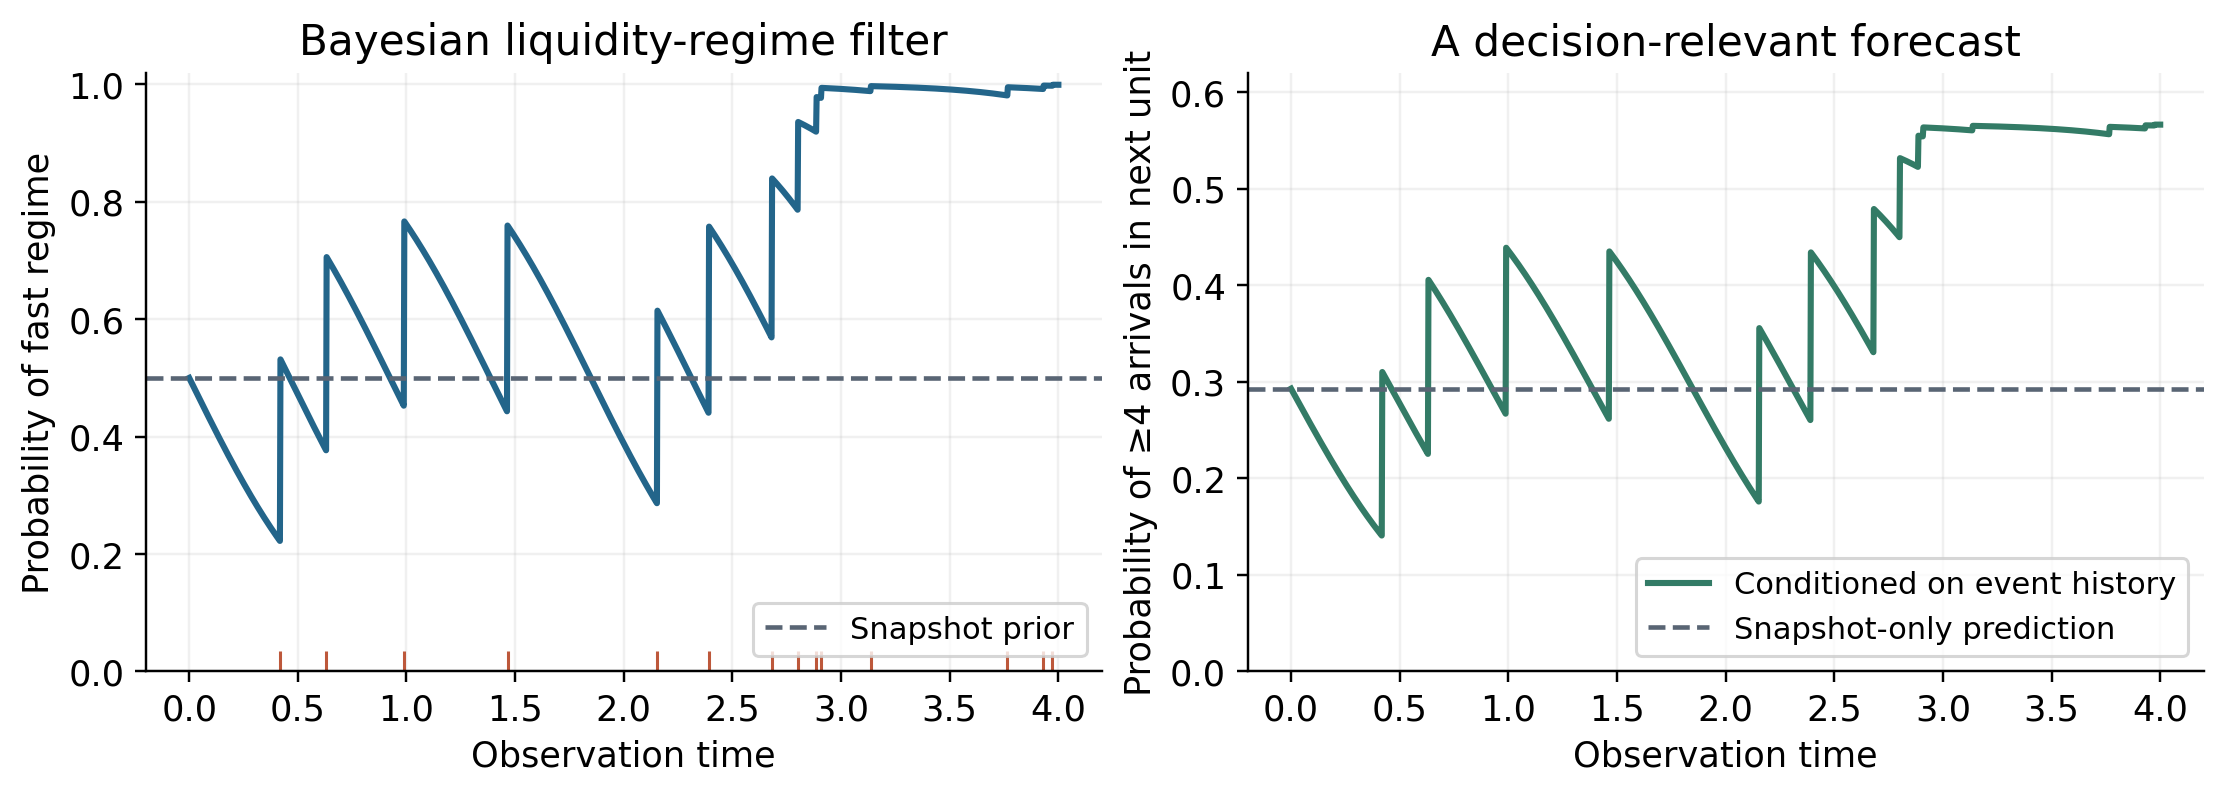
\includegraphics[width=\textwidth]{figures/hidden_liquidity_filter.png}
 \caption{A synthetic fast-regime path and its exact Bayesian filter. Quiet intervals lower the fast-regime probability; arrivals raise it. The right panel shows the resulting forecast for a future arrival-count threshold. The latent regime is not an undepleted hidden reserve.}
 \label{fig:filter}
\end{figure}

\subsection{Exact queue depletion and a path-law certificate}
The second experiment is a continuous-time Markov chain on queue states
$\{0,1,\ldots,6\}$, with state $0$ absorbing. At state $n>0$, the death rate is
$d(n)=1+0.25n$; the birth rate is $1.2$ if $n<6$ and zero at capacity.
The initial state is $4$ and the horizon is $T=2$.
The learned model replaces $d(n)$ by $(1+\theta)d(n)$, leaving births unchanged.

Let $Q$ be the true generator, using row-vector distributions.
Matrix exponentiation gives
$p_T=e_4^\top e^{TQ}$ and the corresponding learned distribution.
The mean-integrated discrepancy is
\begin{equation}
 \E\int_0^T\delta_t\dd t
 =\theta\,e_4^\top\left(\int_0^Te^{tQ}\dd t\right)d
 =3.5212578021\,\theta.
\end{equation}
We evaluate the integral as the upper-right block of
$\exp\bigl(T\left[\begin{smallmatrix}Q&I\\0&0\end{smallmatrix}\right]\bigr)$,
which avoids inverting the singular generator.
The true depletion probability is $0.1693829524$.

\begin{table}[htbp]
 \centering\small
 \begin{tabular}{rrrrrr}
\toprule
$\theta$ & Depl. bias & Terminal TV & $L^1$ bound & KL bound & $|\Delta$CVaR$_{.99}|/B$ \\
\midrule
0.001 & 0.00043 & 0.00061 & 0.00352 & 0.00094 & 0.09379 \\
0.002 & 0.00086 & 0.00122 & 0.00704 & 0.00188 & 0.18753 \\
0.010 & 0.00432 & 0.00611 & 0.03521 & 0.00935 & 0.93514 \\
0.025 & 0.01088 & 0.01522 & 0.08803 & 0.02326 & 1.00000 \\
0.050 & 0.02200 & 0.03024 & 0.17606 & 0.04615 & 1.00000 \\
0.100 & 0.04491 & 0.05962 & 0.35213 & 0.09087 & 1.00000 \\
0.200 & 0.09291 & 0.11544 & 0.70425 & 0.17642 & 1.00000 \\
\bottomrule
\end{tabular}

 \caption{Exact finite-state calculations up to matrix-exponential precision. Depletion bias and terminal TV are measured distributional errors. The $L^1$ and KL columns are full-path TV upper bounds. The final column bounds the absolute CVaR difference divided by cost range $B$, using the smallest available path bound.}
 \label{tab:queue}
\end{table}

At $\theta=0.10$, the depletion probability changes by $0.044909$, terminal TV is $0.059619$, and the mean path bound is $0.352126$. The certificate is conservative but valid. At $\theta=0.20$, the deterministic-envelope bound $0.632121$ is smaller than the mean-integrated bound $0.704252$; either can be used.
For this multiplicative perturbation the exact path KL divergence is
\[
 D_{\rm KL}(P\|\widehat P)=3.5212578021\,[\theta-\log(1+\theta)].
\]
At $\theta=0.10$, Pinsker therefore gives $0.09087$, substantially below the $L^1$ bound while still above terminal TV. At $\theta=0.001$, its 99-percent CVaR error bound is $0.09379B$; at $0.002$, it is $0.18753B$. With the original $L^1$ route alone, a nontrivial 99-percent bound requires $\theta<0.002839894$. The added small-error regimes and likelihood comparison make the informative and vacuous ranges explicit. None of these upper bounds is measured full-path TV.

\subsection{Posterior resolution and a persistent fitting floor}
Take $\mathsf H=L^2(0,1)$ with an orthonormal basis $(e_j)_{j\ge1}$ and target field
\[
 Z=\sum_{j\ge1}\frac{\xi_j}{j}e_j,\qquad \xi_j\stackrel{\rm iid}{\sim}N(0,1).
\]
The learned level-$m$ field has independent coefficients
$[\beta+(1+\eta)\xi_j]/j$ for $j\le m$ and zero coefficients above $m$.
Set $\beta=0.04$ and $\eta=0.06$. Since the covariance operators are diagonal in the same basis, the exact Gaussian Wasserstein error is
\begin{equation}\label{eq:gaussian-posterior}
 \kappa_m^2=\sum_{j>m}j^{-2}
 +(\beta^2+\eta^2)\sum_{j=1}^mj^{-2}.
\end{equation}
This is also the context-independent refinement certificate with $L_j=0$.
For the illustrative density $f_z(u)=1.2+0.4\tanh z(u)$, positivity and
$K=0.4$ hold on $L^2(0,1)$ and $M=1$.
The local posterior-induced rate-error bound is therefore $0.4\kappa_m$.

At $m=256$, $\kappa_m=0.111499$ and the local rate bound is $0.044600$.
The limiting posterior error is $0.092486$, because finer resolution does not remove the bias and variance mismatch in retained coordinates.
This calculation concerns one conditional posterior and its local rate map. Extending it to a complete market path requires the predictable-history assumptions of \Cref{cor:combined}; a one-time Gaussian calculation alone does not establish them.

\begin{figure}[htbp]
 \centering
 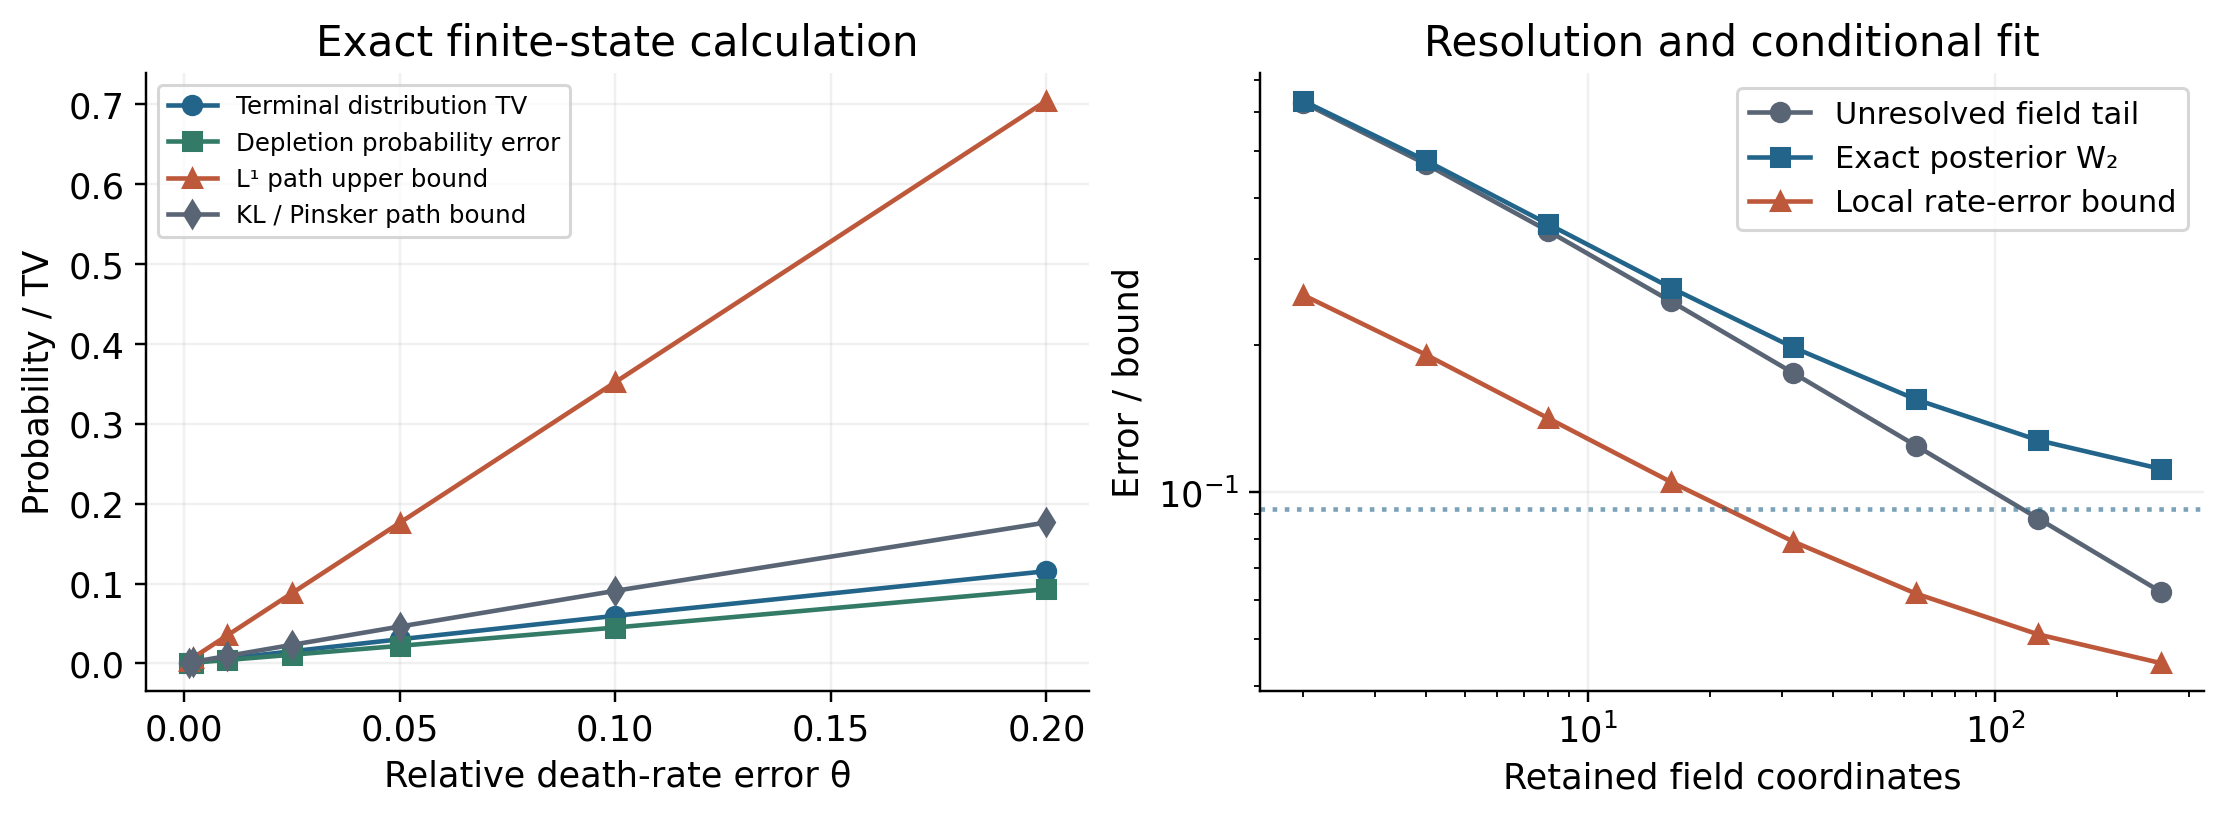
\includegraphics[width=\textwidth]{figures/event_error_certificate.png}
 \caption{Left: exact terminal distribution errors and two full-path upper bounds for the queue chain. Right: the Gaussian posterior calculation \eqref{eq:gaussian-posterior}, its unresolved tail, and the induced local intensity bound. The horizontal dotted line is the persistent posterior fitting floor.}
 \label{fig:certificate}
\end{figure}

\subsection{Liquidity geometry and analytic option prices}
Two static ask books share prices
$(100,100.01,100.03,100.06)$ and have volumes $(2,3,2,3)$ and $(1,2,4,3)$.
Both have ten lots. Their normalized volume transport distance times ten is
$0.05$, exactly the difference between the costs of buying all ten lots.
The partial-quantity costs satisfy \Cref{thm:sweep} at every quantity.

\begin{figure}[htbp]
 \centering
 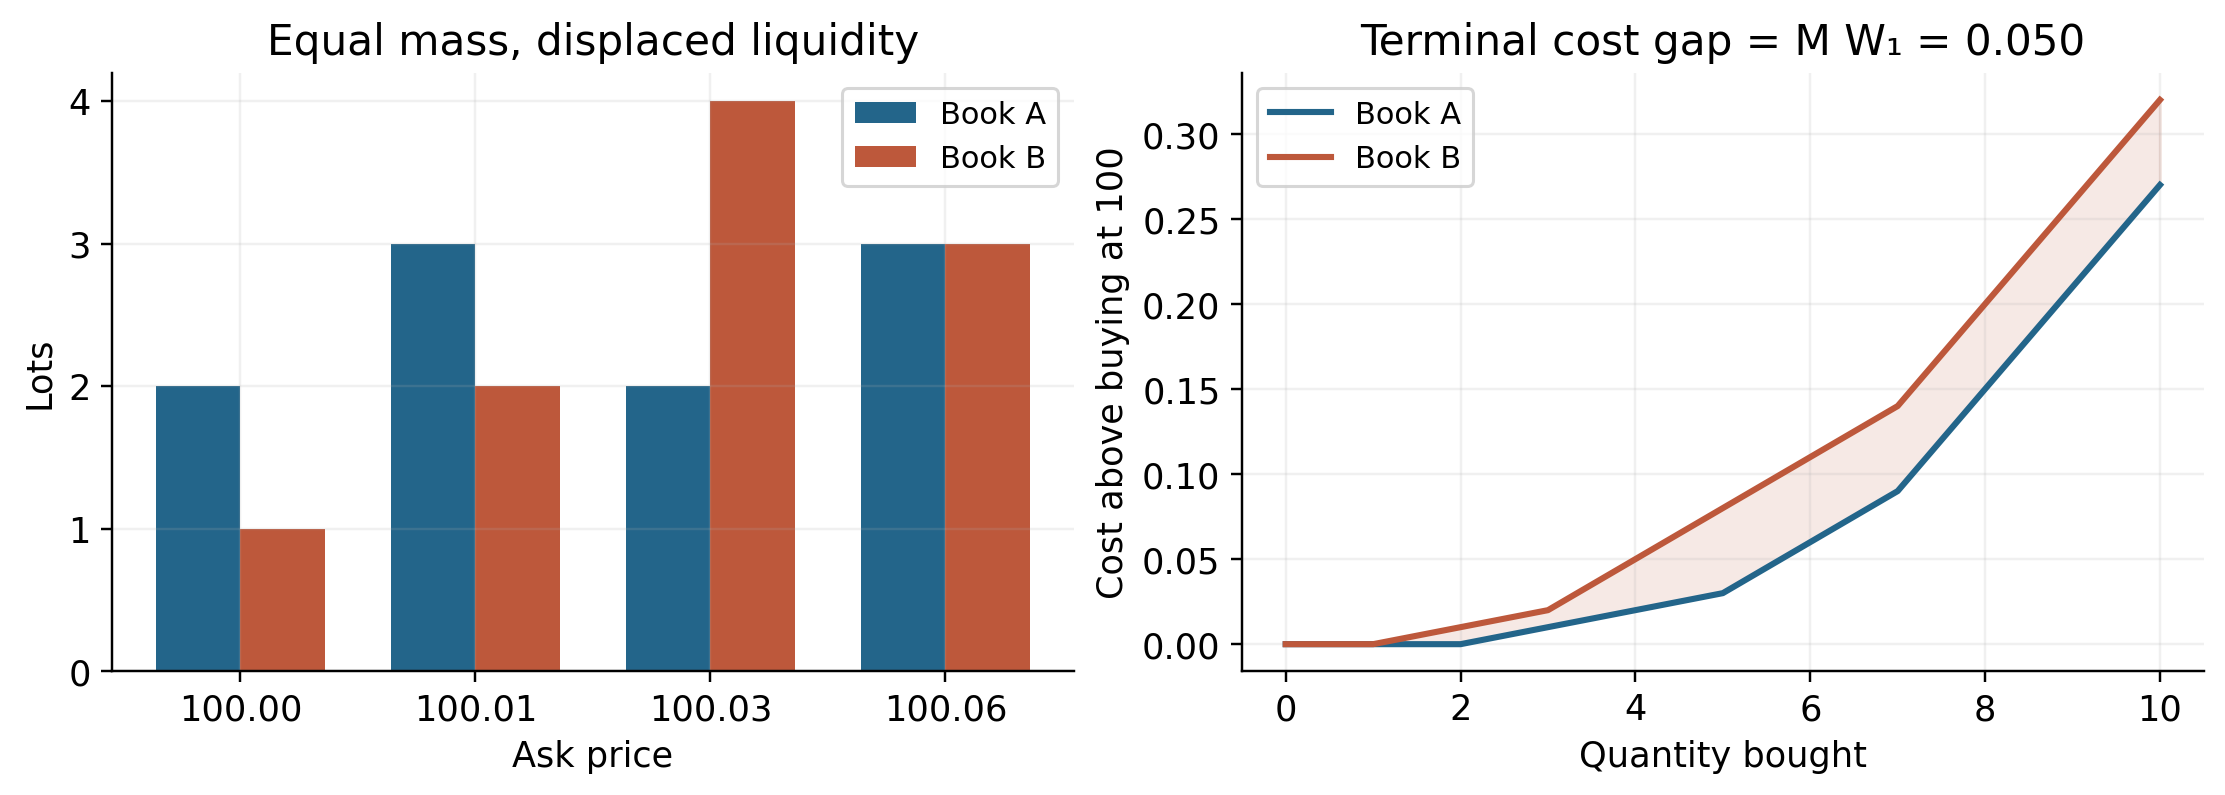
\includegraphics[width=\textwidth]{figures/execution_geometry.png}
 \caption{A sharp static sweep-cost example. The right panel subtracts the common cost $100Q$ to expose the liquidity contribution. The final gap is $0.05$ currency units for ten lots under the stated unit convention.}
 \label{fig:geometry}
\end{figure}

For the pricing illustration, draw a volatility $\sigma\in\{0.15,0.35\}$ with equal probabilities before all return innovations, take $X_0=100$, and use zero interest. Conditional on $\sigma$, use the martingale construction.
Take $\mathcal G_0$ trivial, so the volatility draw is hidden from the market at the pricing origin. The time-zero option price is then the equally weighted mixture of the two analytic lognormal call prices. If the draw is revealed instead, the conditional price is the price for that realized volatility, rather than the mixture.
At-the-money calls at maturities $0.25,0.5,1,2$ have prices
$4.981979$, $7.038809$, $9.935283$, and $13.996948$.
No option-pricing Monte Carlo is needed for these numbers.

\begin{figure}[htbp]
 \centering
 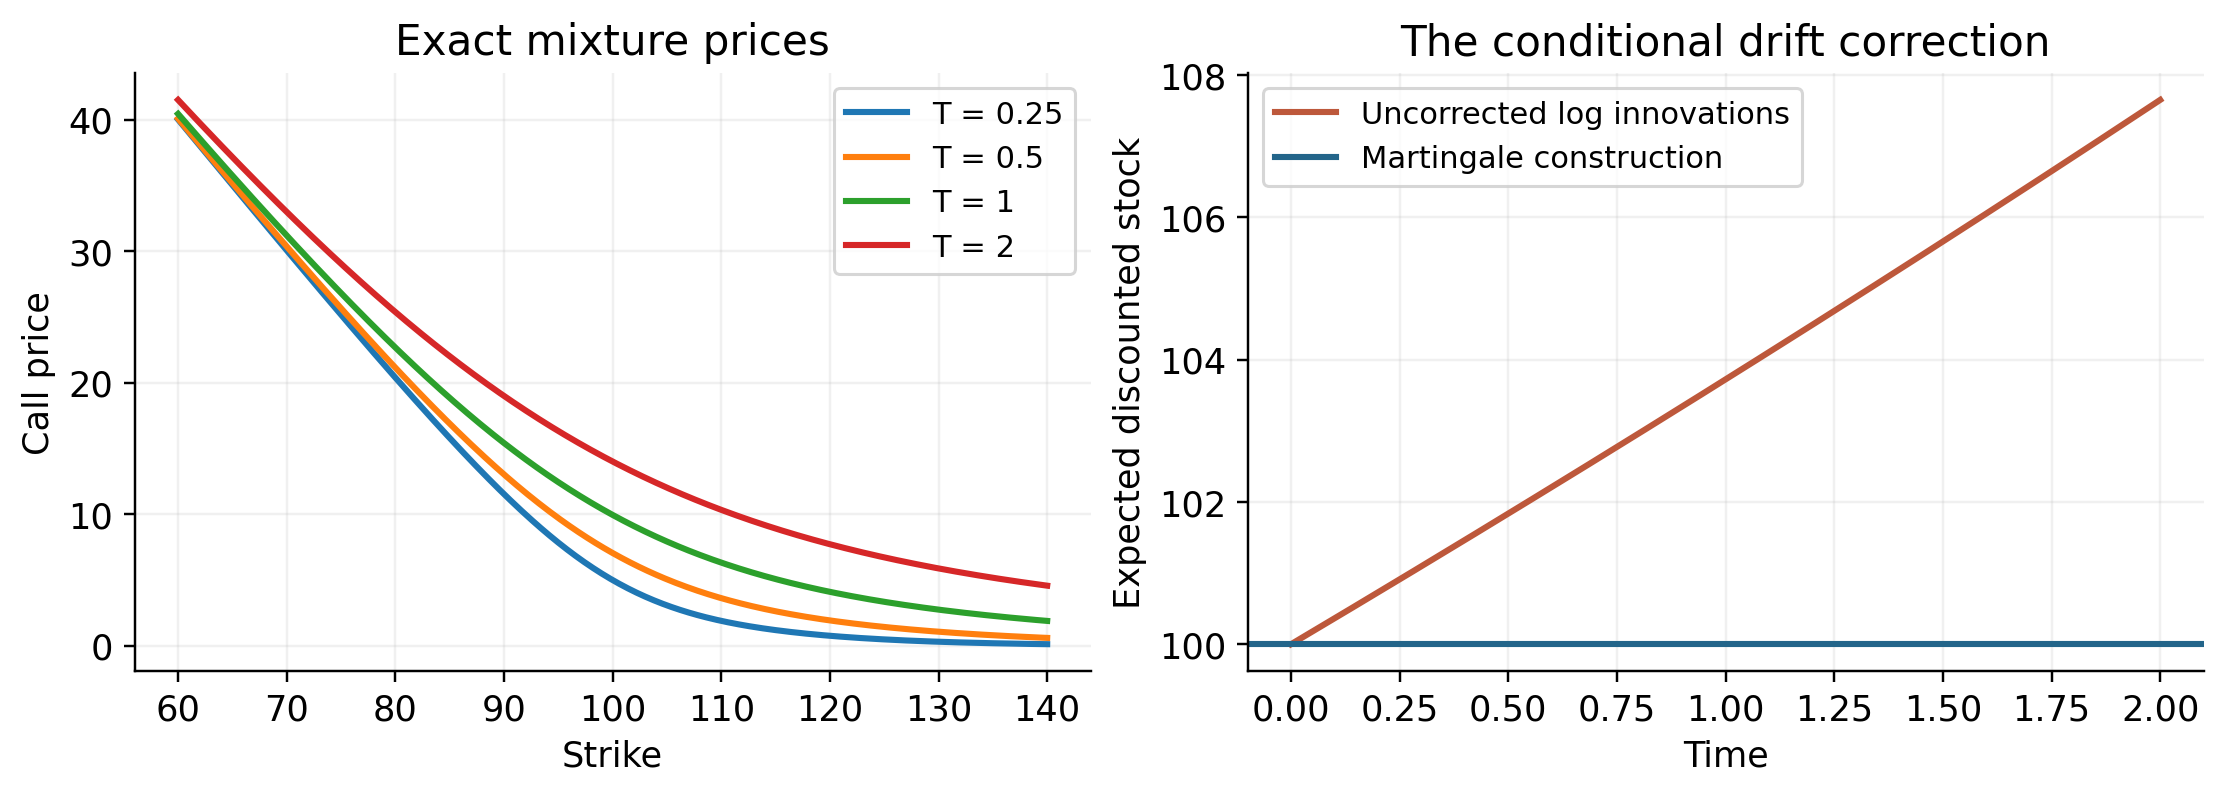
\includegraphics[width=\textwidth]{figures/martingale_pricing.png}
 \caption{A positive mixture martingale with analytic call prices. Omitting the $-\sigma^2T/2$ correction makes the expected discounted stock rise from $100$ to $107.653708$ at $T=2$. Including it keeps that expectation exactly $100$. This is an explicit illustrative generator, not a trained volatility model.}
 \label{fig:pricing}
\end{figure}

\subsection{A complete learned reserve model with an execution decision}\label{sec:complete-model}
This experiment connects hidden inventory, survival-aware filtering, a learned intensity map, exact sampling, and execution evaluation in one model. All rate specifications and labels are synthetic. The model has one displayed ask lot $D=1$, hidden reserve $H\in\{0,\ldots,5\}$, and a fixed hidden regime $R\in\{0,1\}$. Initially $\mathbb P(R=1)=0.4$ and independently $H$ equals $0,2,5$ with probabilities $0.1,0.5,0.4$. This is an explicitly specified aggregate reserve model, not a claim about an exchange's priority rules.

While the trader's passive order is active, the rates are
\begin{equation}\label{eq:complete-rates}
 \lambda_{R,H}=(1+2R)(1+0.08H),\qquad
 \phi_{R,a}=(0.6+0.5a)(0.8+0.4R),\quad a\in\{0,1\}.
\end{equation}
A competing execution consumes the displayed lot. When $H>0$, its mark records a one-lot refresh and updates $(D,H)$ to $(1,H-1)$. When $H=0$, its mark records depletion and the episode ends. An independent passive-fill clock of rate $\phi_{R,a}$ ends the episode with a trader fill. Thus every execution-linked update obeys \eqref{eq:reserve-conservation}. The fill opportunity and its action response are specified parts of this toy market, not inferred counterfactual effects.

The three marks are refresh, depletion, and trader fill. Give each mark a unit-mass event cell; then the conditional rate field is the three-vector
\[
 f(R,H,a)=(\lambda_{R,H}\mathbf1_{\{H>0\}},
          \lambda_{R,H}\mathbf1_{\{H=0\}},\phi_{R,a}),\qquad M=3.
\]
Embed the twelve active hidden states as distinct unit basis vectors in $\R^{12}$. Distinct states are at distance $\sqrt2$. This finite latent geometry accommodates the inventory feasibility indicator directly; no continuous sensitivity is inherited through a discontinuous rounding map.

\paragraph{What is trained.}
A $3$--$24$--$24$--$2$ network with tanh hidden layers and output $10\operatorname{sigmoid}$ receives $(2R-1,H/2.5-1,2a-1)$ and predicts $(\lambda,\phi)$. It has 746 parameters. Training uses all 24 active state/action specifications, with 1,200 Adam updates followed by L-BFGS. The labels are the exact rates in \eqref{eq:complete-rates}; the model is a learned rate emulator, not a market-data estimator. Its finite-domain audit covers every deployed input. This choice isolates whether a learned representation can be inserted into the full probabilistic construction without leaving unmeasured approximation error.

The final mean squared rate error is $4.9514\times10^{-7}$. Exhaustive evaluation gives
\begin{align}\label{eq:complete-constants}
 \epsilon_\lambda&=\max_{R,H,a}\sum_e|f_e-\widehat f_e|=0.00266924,\\
 r_{\max}&=\max_{R,H,a}\|f-\widehat f\|_2=0.00190530,
 \qquad K=3.64972.\notag
\end{align}
Here $K$ is the maximum pairwise learned field difference divided by $\sqrt2$ over required latent states and actions. Both models have total rate below six. The common thinning envelope is therefore $c=6$ on this fully enumerated domain. The analytic bounds are exact mathematical implications; their reported numerical evaluations use float64 and are not interval-arithmetic proofs.

\paragraph{The filter and the decision.}
Before the trader posts, there is no trader-fill clock. For an observed prehistory, the posterior is updated by \eqref{eq:survival-filter}, followed at every refresh by the corresponding likelihood and reserve decrement. We compare three information states: the initial prior; a quiet interval of length $0.5$; and refreshes at $0.1$ and $0.3$ followed by observation through $0.5$. These are specified conditioning histories with positive likelihood density, not selected realized trading records. The neural model uses its own rates to compute its posterior on the same history.

After the two refreshes, the true posterior mean reserve is $1.417759$ and the fast-regime probability is $0.648446$. Dropping survival information gives posterior TV error $0.208696$. The correctly updated neural posterior has TV error $7.97\times10^{-5}$. A direct likelihood calculation over initial states verifies the recursive filter to $5.6\times10^{-17}$.

The trader selects an action $a\in\{0,1\}$ and deadline $\tau\in\{0,0.1,\ldots,1.5\}$. A passive fill costs $0.04a$, depletion before fill costs $1$, and crossing at the deadline while still active costs $0.3$. Costs are per lot in a declared currency unit, with $B=1$. The finite class has 32 configurations and is optimized by enumerating their expected costs. It is a deadline policy class, not the unrestricted solution of a partially observed control problem.

The full model is a 14-state CTMC: twelve active hidden states and two absorbing outcomes. If $p$ is the posterior at the decision origin, $p^Te^{\tau Q_a}$ gives its exact outcome probabilities up to matrix-exponential numerical precision. A neural posterior $\widehat p$ and generator $\widehat Q_a$ give the corresponding model values. No path Monte Carlo is used to choose or value these policies.

\begin{table}[htbp]
\centering\small
\begin{tabular}{lrrrrr}
\toprule
History & Action & Deadline & True cost & Max. value error & Path bound \\
\midrule
initial & 1 & 1.5 & 0.244577 & 1.75e-05 & 4.00e-03 \\
quiet & 1 & 1.5 & 0.223617 & 2.99e-05 & 4.06e-03 \\
two refreshes & 0 & 0.0 & 0.300000 & 7.50e-05 & 4.08e-03 \\
\bottomrule
\end{tabular}

\caption{Exact finite-state policy evaluation. The maximum value error is over all 32 policies at the stated history. The final column is a uniform full-path certificate for the entire deadline class; it is not measured path TV.}\label{tab:complete-model}
\end{table}

Write $\delta_0=\TV(p,\widehat p)$. Couple these initial hidden states maximally and then apply common-event thinning. For every policy in the class,
\begin{equation}\label{eq:complete-path}
 \TV(P^a,\widehat P^a)\le
 1-(1-\delta_0)e^{-1.5\epsilon_\lambda}.
\end{equation}
This gives the final column of \Cref{tab:complete-model}. The same argument bounds the joint hidden-state/history laws at each earlier time, so \Cref{prop:filter-stability} and the $W_1$ version of \Cref{lem:posterior} also give the separate field/posterior certificate
\begin{equation}\label{eq:complete-field}
 \sqrt3\left[1.5r_{\max}
 +2\sqrt2K\int_0^{1.5}\{1-(1-\delta_0)e^{-\epsilon_\lambda t}\}\dd t\right].
\end{equation}
Its values are $0.05857$, $0.06021$, and $0.06070$. The direct full-state coupling is substantially tighter in this small enumerated model. Reporting both shows the price of the representation-level decomposition; it does not conceal it behind the abstract theorem.

The learned and true models select the same policy in each information state, giving zero regret within the enumerated class. After the prior or quiet history, action $1$ with deadline $1.5$ is preferred; after two refreshes, immediate crossing is preferred. The uniform regret bounds are about $0.0080$--$0.0082$ currency units. The corresponding 99-percent CVaR error bounds are $0.3996$--$0.4075$ units, below the trivial bound $B=1$. Several actual policies have CVaR equal to the worst cost; a nontrivial bound is not evidence that their tail losses are small.

\paragraph{Sampling independently checked.}
We implement both exact averaging and one fresh posterior draw per proposal, updating the entire belief after accepted marks. In 20,000 paths for each method, with action $1$, horizon $0.8$, and the two-refresh posterior, all three terminal probabilities agree with matrix exponentiation within five binomial standard errors. Maximum absolute discrepancies are $0.00356$ and $0.00739$. These are sampling diagnostics; exactness of the construction follows from \Cref{prop:posterior-thinning}.

\begin{figure}[htbp]
\centering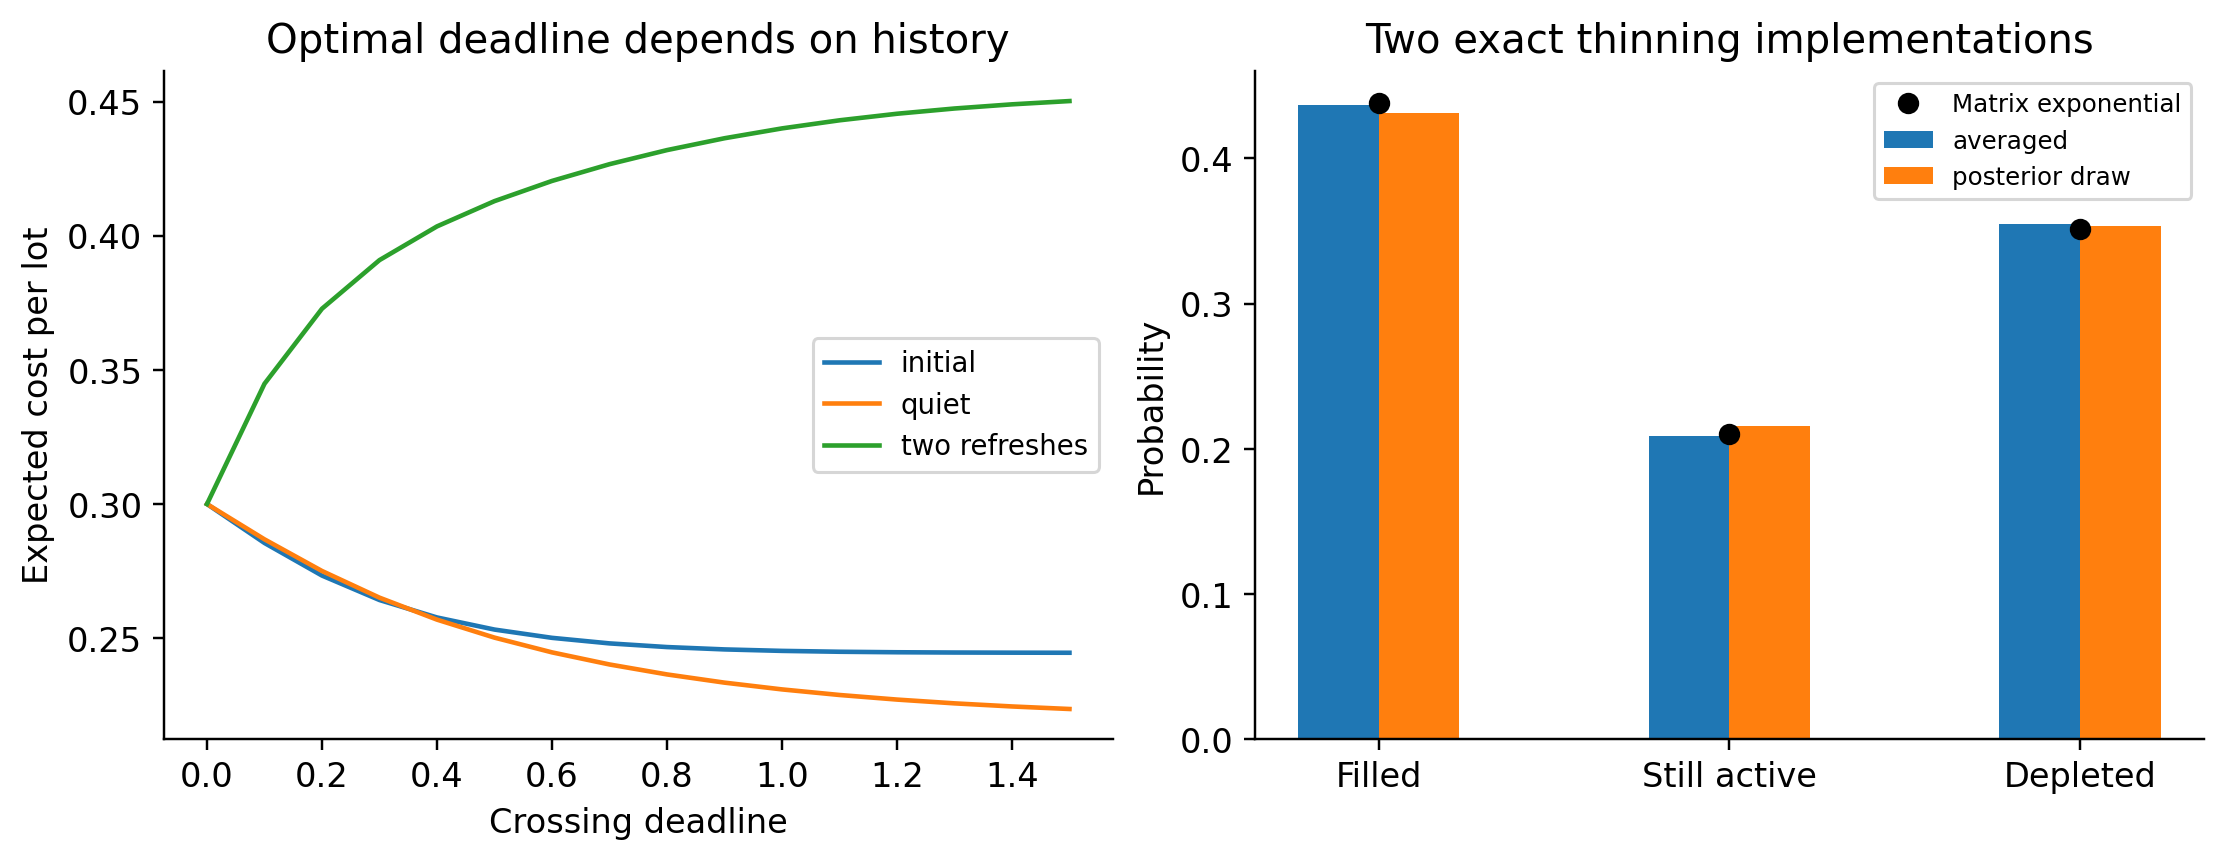
\includegraphics[width=\textwidth]{figures/learned_reserve.png}
\caption{Left: true expected execution cost, minimized over the two action choices at each deadline, for three observed histories. Right: two thinning implementations compared with independently computed CTMC outcome probabilities.}\label{fig:complete-model}
\end{figure}

\subsection{A genuinely adapted volatility perturbation}
To test \Cref{thm:vol-price}, use 32 equal steps over $T=1$ and let
\[
 W_n=\sum_{k<n}\sqrt{\Delta_k}Z_{k+1},\qquad
 \sigma_n=0.2+0.1\tanh(W_n),\qquad
 \widehat\sigma_n=\sigma_n+\delta.
\]
Both volatilities are selected before the next return innovation. For
$\delta\in\{0.005,0.01,0.02\}$, take the common bound $\bar\sigma=0.32$.
The theorem input is exactly $\mathcal A_N=\delta^2$, not an estimated future-path transport distance. From 200,000 common-innovation paths with $X_0=100$, the at-the-money call differences are $0.199253$, $0.398629$, and $0.797714$, with standard errors $0.000892$, $0.001789$, and $0.003602$. The improved deterministic bounds are $0.694672$, $1.389344$, and $2.778688$. Estimated absolute terminal coupling errors are $0.400444$, $0.800891$, and $1.601781$. The bound controls these coupled constructions and Lipschitz payoffs; it is not an assertion that this coupling realizes $W_1$.

\subsection{Learning from event counts and selecting a certified policy}
The reserve experiment tests the partially observed simulator with a specified latent model. A separate finite observable example tests the statistical and control results of \Cref{sec:certified-control} using event data alone. Its role is to isolate what can be certified when state-action exposure is actually observed.

The state is $(q,z)$ with remaining quantity $q\in\{0,1,2,3,4\}$ and observed regime $z\in\{0,1\}$. The actions are passive ($a=0$) and aggressive ($a=1$). A fill reduces $q$ by one; a regime mark changes $z$ to $1-z$. States with $q=0$ are absorbing. For positive quantity the synthetic rates are
\begin{align}\label{eq:control-truth}
 \lambda_{\rm fill}(q,z,a)&=(0.75+0.10q)(1+0.35z)(1+1.8a),\\
 \lambda_{\rm regime}(q,z,a)&=0.35+0.10q+0.12a+0.20z.\notag
\end{align}
Their known envelopes are $5$ and $1.5$. At horizon $T=2$, the terminal cost is $q(1+0.2z)$; running cost is $0.03q^2$; a passive fill costs $0.03$ and an aggressive fill costs $0.35$. Regime changes have no direct cost. This fully specified objective measures an execution trade-off, without purporting to reproduce an exchange fee schedule or empirical spread process.

Each observed episode starts with randomized positive quantity and regime. A behavior action is chosen independently at the initial state and after each event, and held until the next event or horizon. The recorded sufficient statistics are the event counts and occupation times for every state-action-mark triple. Three independent streams use seeds $5101,5102,5103$ and prefixes of $2{,}000$, $8{,}000$, and $32{,}000$ episodes. The rate intervals use sixteen geometrically spaced positive $\eta$ values between $0.005$ and $1$, with the 1\% failure budget divided across the three streams. Time-uniform coverage includes every prefix without an additional prefix penalty. The 32 active triples, confidence endpoints, exposures, and counts are serialized.

A $3\to12\to2$ tanh network with sigmoid rate outputs has 74 parameters. Its inputs encode quantity, regime, and action, and its output envelopes are the known rate caps. Training uses $1{,}400$ Adam steps on the exposure-weighted negative log-likelihood
$\sum_i\{\widehat\lambda_i E_i-N_i\log\widehat\lambda_i\}$.
The true rates in \eqref{eq:control-truth} are never training labels. The deployed rate vector is clipped to the confidence box, with the raw network output also retained. The nominal neural policy minimizes its estimated cost. The robust policy minimizes the upper Hamiltonian over the whole box; its guarantee does not depend on successful network optimization. This separation makes it possible to assess both learned predictions and uncertainty-aware decisions.

Both robust equations use $8{,}000$ time steps and the residual allowance in \Cref{prop:control-residual}. The true costs of the resulting feedback policies are computed by matrix exponentiation over runs of identical action vectors. This evaluates the actual continuous-time policy, including possible changes of action at grid boundaries. A high-accuracy DOP853 solution computes the known-model optimum, independently cross-checked against a $16{,}000$-step Euler solution and its residual allowance. Truth enters these diagnostics, not the data-derived confidence box or robust decision.

\begin{table}[htbp]
\centering\small
\begin{tabular}{rrrrr}
\toprule
Episodes & Neural regret & Robust regret & 99\% regret bound & Time residual \\
\midrule
2,000 & 0.00214 & 0.02138 & 1.0618 & 0.0104 \\
8,000 & 0.00014 & 0.00657 & 0.4681 & 0.0105 \\
32,000 & 0.00004 & 0.00161 & 0.2341 & 0.0102 \\
\bottomrule
\end{tabular}

\caption{Execution from initial state $(4,0)$. The neural and robust regrets are means over the three fixed data streams, evaluated against the known synthetic optimum. The confidence column is the largest theorem-derived bound across those streams, including time discretization; the final column is the largest sum of numerical residual allowances. Confidence refers to the analytic event, not a formally rounded floating-point enclosure.}\label{tab:certified-control}
\end{table}

The known optimum is $1.733392$. At $32{,}000$ episodes, robust-policy regret ranges from $0.001178$ to $0.001968$, while its certificate ranges from $0.226235$ to $0.234137$. All true rates fall inside their intervals in the reported runs; this observed coverage is a diagnostic, not a substitute for the simultaneous theorem. The nominal neural policy has lower realized regret in these examples. Robustness therefore has a measured conservatism cost; these experiments do not claim that pessimism always improves realized performance. Rectangular uncertainty and protection against every admissible rate vector explain part of the gap between measured regret and its bound.

\begin{figure}[htbp]
\centering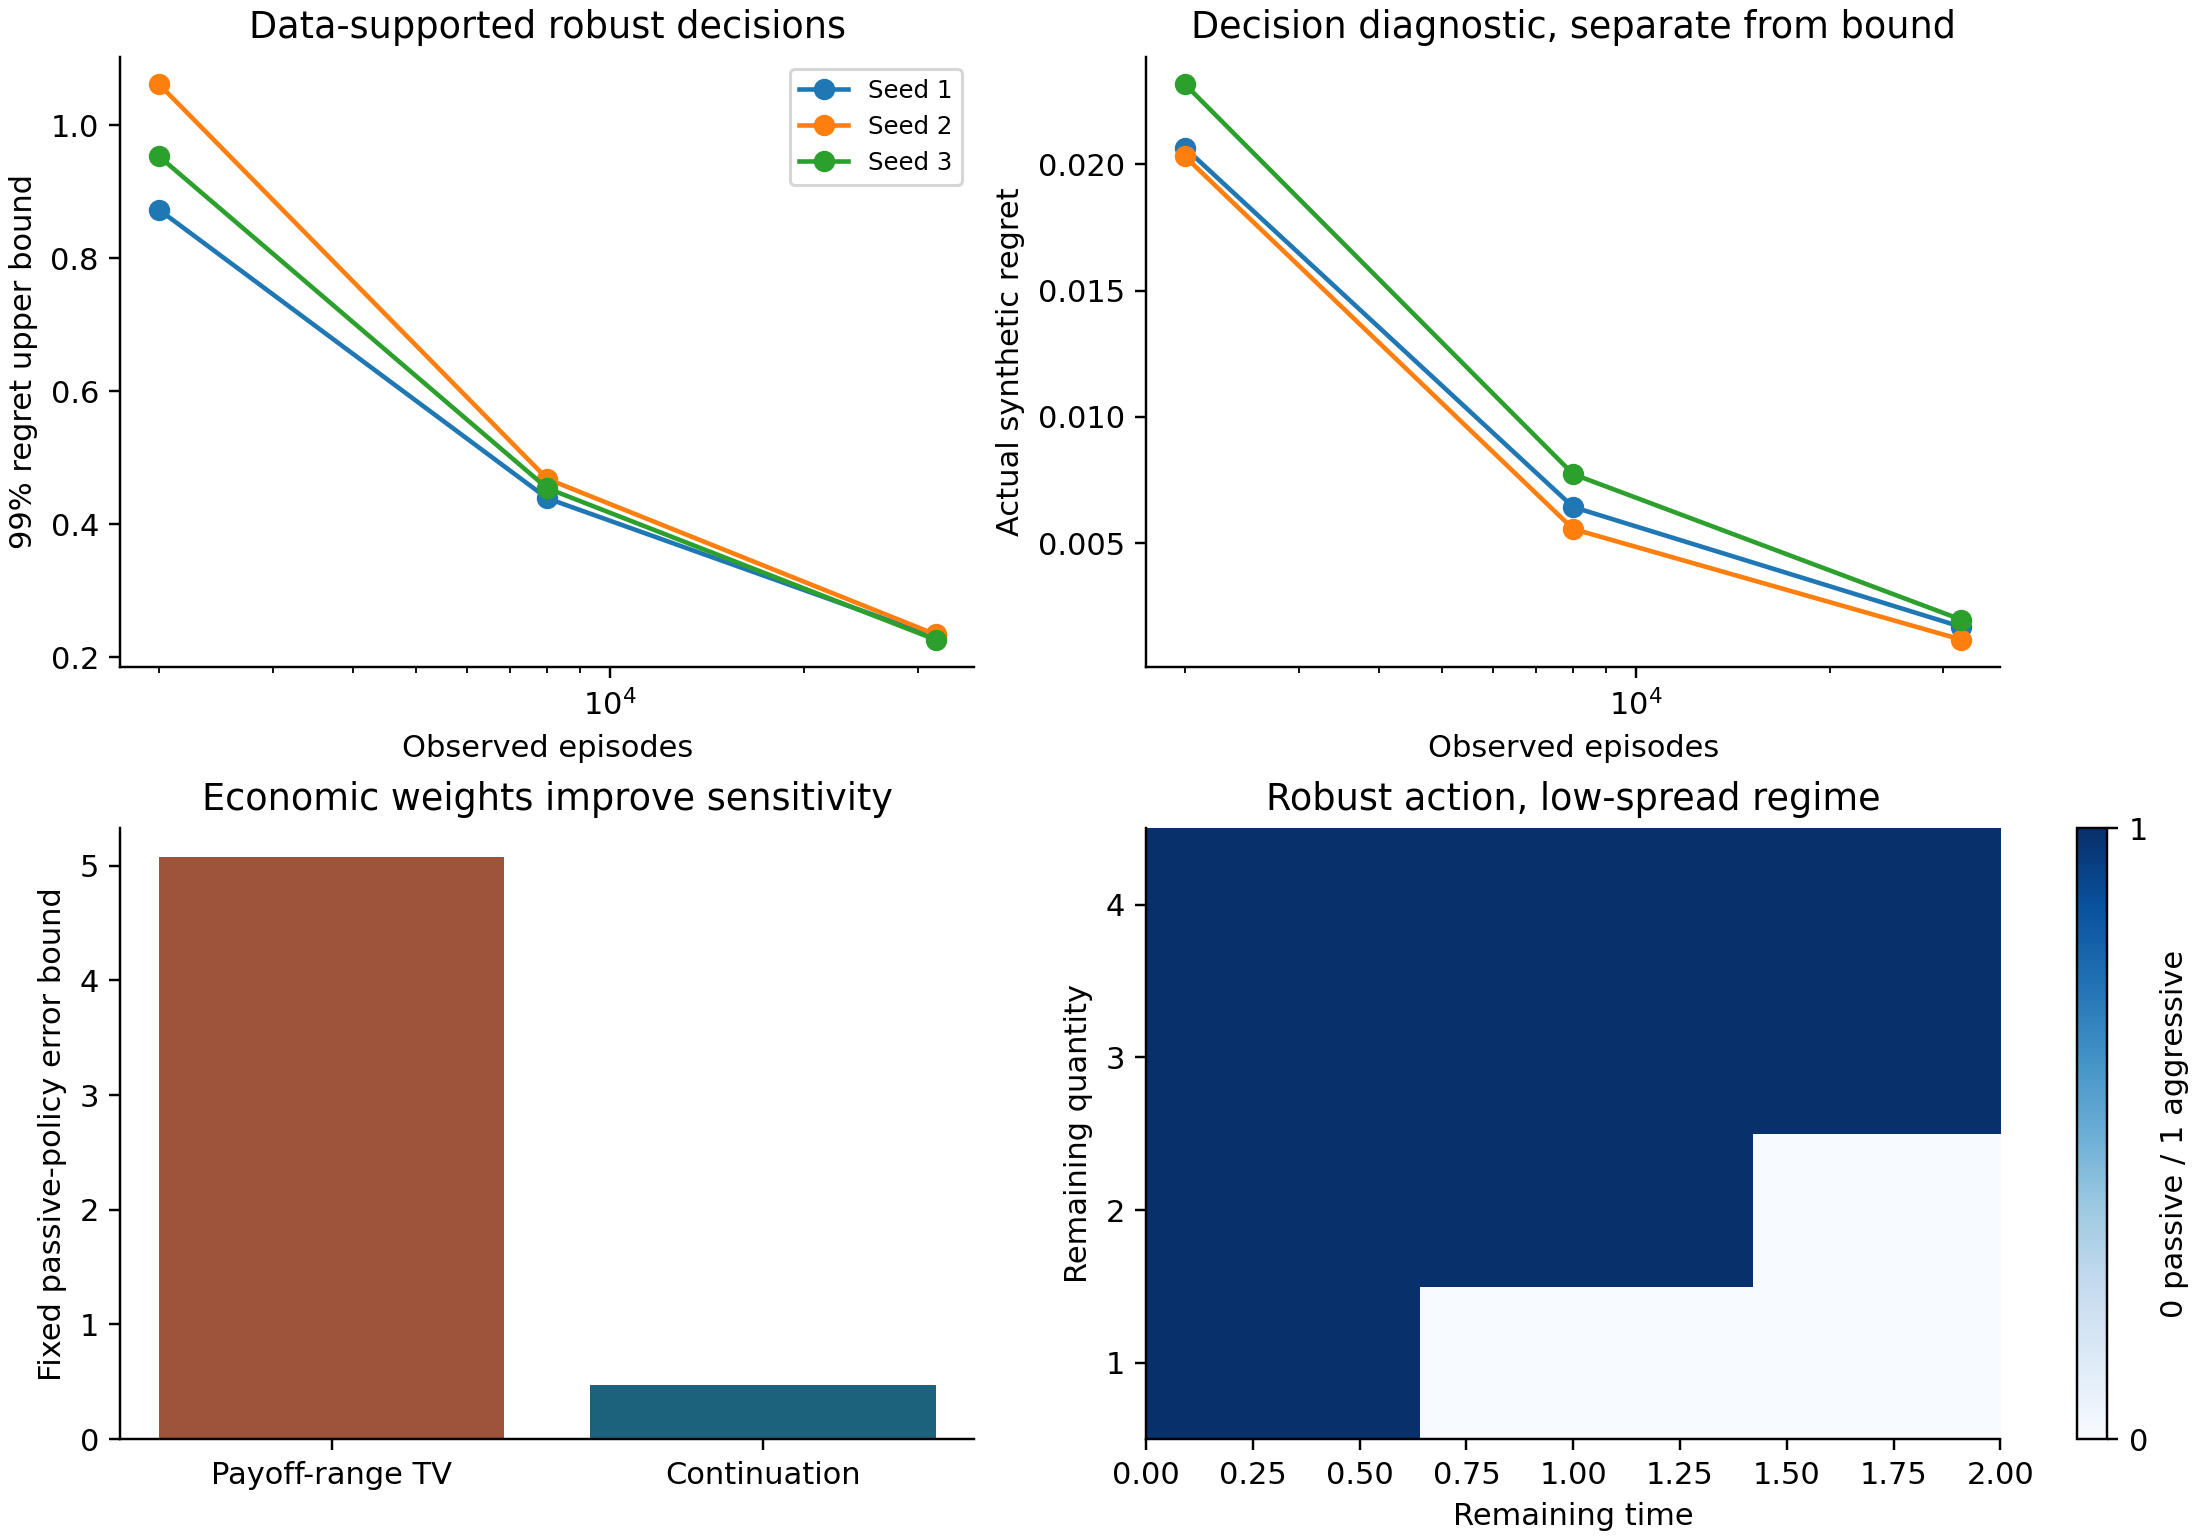
\includegraphics[width=\textwidth]{figures/certified_control.png}
\caption{Observed-event learning and decision certification. Upper panels separate the simultaneous regret bound from actual synthetic regret. Lower left compares two uncertainty bounds for a fixed passive policy. Lower right shows the robust feedback action at the largest data budget of the first stream.}\label{fig:certified-control}
\end{figure}

\subsection{Sensitivity and numerical error in the same decision model}
For the fixed passive policy in the first stream's largest dataset, the exact true-minus-learned cost difference is $-0.00904582$. Numerical integration of the signed continuation identity differs by only $4.82\times10^{-9}$. The statewise continuation bound is $0.469600$, compared with $5.071310$ from the payoff-range times path-TV route using the same rate intervals. Their ratio is about $10.80$. The comparison is objective-specific; a different payoff can assign very different weights to the same events. The continuation integral is numerically evaluated on 2,001 time points and is not claimed to have a rigorous quadrature enclosure.

Doubling the upper-control grid from $8{,}000$ to $16{,}000$ steps changes its initial value by $7.32\times10^{-5}$. The corresponding analytic residual allowances are $0.004900$ and $0.002450$. This check supports the implementation and expected first-order refinement. The allowance bounds the continuous-time interpolation error in exact arithmetic; the program labels its floating-point results accordingly.

Finally, the equal-terminal-law example in \Cref{ex:early-information}, evaluated at $r=0.1$, has early-revelation American value $0.452419$ and late-revelation value $0.409365$. The European values coincide at $0.409365$. The calculation isolates information timing, which neither terminal-law calibration nor an arbitrary path coupling can remove.


\subsection{Reproducibility and limits of the calculations}
The initial Python program regenerates four PNG figures, the queue table, and its JSON results. The reserve and observed-control programs add their respective figures, tables, learned parameters, and full diagnostic records. Each program records its seeds and software versions. It checks the filter against an independent Bayes calculation; generator row sums and integrated occupation time; probability and terminal-TV inequalities; the sharp sweep-cost example; call monotonicity and convexity on the reported grid; and reserve conservation and nonnegativity over 784 admissible integer event combinations.

These are useful consistency checks, but they are not proofs of the continuous statements. The Lean project verifies selected universal statements exactly, while the manuscript proves the analytic results. The new reserve experiment trains a rate network on known synthetic specifications, audits every deployed state/action, and compares exact decision values. The other illustrations remain explicit mathematical examples. No exchange-data calibration or investment-performance claim is made.

\section{Formal verification and remaining analytic obligations}\label{sec:lean}
The accompanying project uses Lean 4.19.0 and the matching pinned mathlib release
\citep{demoura2021,mathlib2020}. It contains 40 theorem declarations with checked proof terms. The count includes supporting lemmas and the refinement results also used in the general operator paper; it is not a count of new mathematical contributions.

\subsection{Finite probability and executable market accounting}
The Lean structure \texttt{FiniteLaw} contains a function assigning a real mass to each outcome of an arbitrary finite type, a proof that all masses are nonnegative, and a proof that they sum to one. Expectations and total variation are defined from those masses, with
$\TV(P,Q)=\frac12\sum_i|p_i-q_i|$.
The project proves total variation's nonnegativity, symmetry, and triangle inequality. It then proves
\[
 \left|\sum_ip_iC_i-\sum_iq_iC_i\right|\le B\TV(P,Q)
 \quad\text{whenever }0\le C_i\le B.
\]
The argument subtracts $B/2$ from the payoff and uses equal total mass, preserving the sharp range constant $B$. Indicator payoffs give the event-probability bound. These are the finite-law versions of \Cref{thm:risk}, not an encoding of continuous-time event-path measures.

The reserve module contains an executable transition that accepts an event only when the execution fits displayed inventory and the replenishment fits hidden inventory. It returns either a new pair of natural-number inventories or rejection. Lean proves that every accepted event satisfies
$D'+H'+q=D+H$, and that every accepted finite replay satisfies
\[
 D_{\rm final}+H_{\rm final}+\sum_kq_k=D_{\rm initial}+H_{\rm initial}.
\]
This verifies conservation with natural-number subtraction and explicit rejection of invalid quantities. It does not purport to formalize a complete exchange's allocation, priority, or refresh rules.

\subsection{Finite histories and posterior acceptance}
The path-law module constructs a normalized joint law from a finite history distribution $P$ and a conditional next-mark kernel $K$, with mass $p(x)K(x,e)$. It proves directly from these masses that
\[
 \TV(P\otimes K,Q\otimes L)
 \le\TV(P,Q)+\sum_xp(x)\TV(K(x),L(x)).
\]
It then recursively constructs distributions on complete finite histories, retaining every mark. If the conditional next-mark discrepancies are at most $\epsilon_n$ on every history, Lean proves
\[
 \TV(P_{0:N},Q_{0:N})\le\sum_{n<N}\epsilon_n.
\]
This is a finite discrete-step path theorem, not a terminal-state comparison. It remains distinct from the manuscript's continuous-time event-path theorem; simply rounding continuous event times would not justify applying it to that law.

For posterior thinning, Lean also proves that the finite acceptance probability
$\sum_sp_s\lambda_s/c$ lies in $[0,1]$ when $0\le\lambda_s\le c$ and $c>0$, and that multiplying by $c$ gives $\sum_sp_s\lambda_s$. The marked-Poisson compensator argument in \Cref{prop:posterior-thinning} supplies the continuous-time interpretation.

\subsection{Geometry, risk, and pricing declarations}
The finite cell-integration theorem bounds the sum of absolute cell-rate errors by the weighted absolute field error. A second theorem proves the weighted Cauchy--Schwarz estimate
\[
 \sum_iw_i|d_i|
 \le\sqrt{\sum_iw_i}\sqrt{\sum_iw_id_i^2},
 \qquad w_i\ge0,
\]
including zero weights. Thus the finite quadrature constant is the square root of reference mass, rather than automatically the square root of coordinate count.

The execution module proves a discrete price-quantile prefix inequality, the uniform policy comparison against every comparator, and the finite-law CVaR auxiliary-objective error before the infimum over its threshold. The pricing module proves the positivity of the finite normalizer in \Cref{prop:finite-martingale}, positivity of all normalized returns, their exact mean-one identity, and preservation of the conditional stock mean. No sampled approximation to a normalizing expectation is used in these formal statements.

The refinement module checks the same real-valued radius recursion used in \Cref{thm:posterior-certificate}. It proves the nonlinear comparison, the linear majorant, the exponential bound, and the exact context-independent identity. Its input is the squared one-step discrepancy inequality; the probabilistic construction establishing that input is outside the Lean module.

\begin{table}[htbp]
\centering\small
\begin{tabularx}{\textwidth}{@{}p{.29\textwidth}X@{}}
\toprule
Mathematical component & Checked scope\\
\midrule
Reserve accounting & Executable natural-number transition, rejection, and finite replay conservation.\\
Path laws and sampling & Normalized history/mark composition, conditional TV bound, full finite-history error accumulation, and posterior acceptance identity.\\
Field-to-rate geometry & Finite cell aggregation and weighted $L^1$--$L^2$ inequality.\\
Posterior refinement & Real-sequence comparison and finite exponential certificate.\\
Execution and risk & Finite-law bounded payoff and event inequalities; finite CVaR auxiliary objective; universal value-function regret comparison.\\
Static liquidity & Discrete quantile-prefix bound; no formal identification with $W_1$.\\
Pricing & Finite categorical mean normalization and one-step mean preservation.\\
Decision certification & Rate-box endpoint inequalities, comparator-specific regret, finite probabilistic Bellman sandwich, and accumulated residual bound.\\
\bottomrule
\end{tabularx}
\caption{Formal coverage of the finance project. The continuous-time and infinite-dimensional results remain analytic proofs in the manuscript.}
\end{table}

\subsection{Finite probabilistic control and numerical residuals}
The certified-control module proves sign-dependent rate-box endpoint bounds and the comparator-specific inequality \eqref{eq:pessimistic-oracle}. It also defines an actual finite-horizon policy value recursively from normalized transition laws and costs. Expectation monotonicity proves that a Bellman subsolution for every action bounds every policy from below, while a supersolution for a selected action bounds that deployed policy from above. A separate theorem proves that local Bellman residuals accumulate by their sum, using the sup-norm nonexpansiveness of probability-weighted expectation. These are universal finite-probability statements, not arithmetic checks of one experimental table.

The relation to \Cref{thm:robust-policy,prop:control-residual} is an explicit discrete-time analogue. Continuous-time HJB comparison, the Dynkin identity, counting-process supermartingales, simultaneous rate confidence, and bicausal stopping-time transfer remain manuscript proofs. The encoded finite transition law is normalized by construction; the formal statements do not silently assume that an arbitrary unnormalized numerical matrix is a probability kernel.

\subsection{The analytic boundary and independent reproduction}
The project does not formalize the compensator identity, construction of common Poisson random measures, maximal path coupling, disintegration, measurable selection of optimal transport plans, the Hilbert-valued infinite limit, the full CVaR infimum theorem, or the Gaussian martingale and adapted volatility-to-price estimates. The manuscript supplies those proofs under explicit hypotheses. None is inserted into the Lean project as an unproved axiom.

\begin{samepage}
From the supplied \texttt{lean/} directory, the standard commands are
\begin{verbatim}
lake exe cache get
lake build
lake env lean Audit.lean
\end{verbatim}
\end{samepage}
The package includes the exact dependency manifest, a declaration-level coverage map, build and axiom-audit logs, and a verification script recording source hashes.
No proof uses an admission or a custom mathematical axiom. The axiom audit identifies only the standard logical foundations needed by the declarations. A small executable-location compatibility adjustment used in the build environment is documented separately; it does not modify the proof kernel.

Formal validity of the encoded mathematics does not establish historical calibration, latent-inventory identifiability, correctness of a production matching engine, or the prerequisites for counterfactual policy evaluation. Those are separate scientific and engineering claims.

\section{Discussion and further research}\label{sec:discussion}
The central connection is between a law on latent fields and the law of observable events. Integrating intensities gives a norm with stable resolution constants; conditional transport controls latent uncertainty; common-event coupling handles discontinuous market transitions; and total variation controls bounded execution and risk functionals. Each component addresses a different failure mode.

Several conditions determine whether this theory can become a useful learned financial model. First, the event representation must reconstruct the state needed by the transition rule. A displayed-depth snapshot, an order-level queue, and a trade-and-quote stream contain different information. Latent variables can summarize missing information, but their physical interpretation remains conditional on the structural model. Second, the learned belief must remain accurate along the histories encountered in use. A local posterior approximation does not prove stability of a nonlinear filter through a long sequence of observations.

Third, the intensity sensitivity can be the limiting factor. A highly accurate field reconstruction may be insufficient if a hidden decoder turns small coordinate changes into large changes in feasible event rates. In such cases one should compare the observable conditional rate vectors directly, use a latent metric matched to their predictive equivalence, or retain a discrete latent state with a suitable probability metric. The Hilbert formulation is a design option with explicit assumptions, not a universal coordinate system for integer market state.

Fourth, policy evaluation requires intervention-aware dynamics. \Cref{thm:rate-confidence,thm:robust-policy} give a complete event-data certificate in an observable finite-state model with predictable behavior actions and sufficient exposure. They do not supply latent exposures or correct an omitted state variable. The uniform bound in \Cref{thm:regret} describes what must be established for a policy class; it does not establish that condition from passive records. A strong empirical study would therefore compare a displayed-only predictor, a point-estimate latent predictor, and a posterior-aware model under the same observation and action regime. It would report likelihood, event-validity rates, conditional fill and depletion probabilities, execution-cost calibration, and stress behavior, with uncertainty intervals and chronological evaluation splits.

For pricing, an adapted positive martingale offers exact financial structure but does not determine the economically appropriate pricing measure. Calibration to option quotes and dynamic consistency of additional traded instruments remain separate tasks. The volatility-to-price estimate identifies a coupling error that can be meaningful for a sequential generative model, while showing why arbitrary future-path transport is insufficient.

The stopping-time comparison additionally requires preservation of the observed information structure. The equal-terminal-law example shows that terminal calibration can coexist with an exercise-value discrepancy.

Open problems include rate confidence regions for partially observed histories, stability of learned posterior approximations, joint rather than rectangular rate uncertainty, sharper decision-specific bounds, and empirically justified counterfactual dynamics. The finite observable experiment provides a benchmark where these components can be separated; applying the full latent-field theory to exchange records requires additional identification and calibration evidence.

\FloatBarrier
\bigskip
\phantomsection
\addcontentsline{toc}{section}{References}
\bibliographystyle{plainnat}
\begingroup
\interlinepenalty=10000
\setlength{\bibsep}{3pt}
\bibliography{references}
\endgroup
\end{document}
